\documentclass[11pt]{article}
\usepackage[a4paper,margin=1in]{geometry}
\usepackage{amsmath,amssymb,amsthm}
\usepackage{booktabs}
\usepackage{microtype}
\usepackage{xcolor}
\usepackage{hyperref}
\usepackage{graphicx}
\usepackage{caption}
\usepackage{subcaption}
\usepackage{enumitem}

\graphicspath{{../main/visualizations/}}

% ---- Theorem environments ----
\newtheorem{theorem}{Theorem}[section]
\newtheorem{proposition}[theorem]{Proposition}
\newtheorem{corollary}[theorem]{Corollary}
\newtheorem{lemma}[theorem]{Lemma}
\theoremstyle{definition}
\newtheorem{definition}[theorem]{Definition}
\newtheorem{remark}[theorem]{Remark}
\newtheorem{conjecture}[theorem]{Conjecture}

% ---- Operators / notation ----
\DeclareMathOperator{\occ}{\#}
\newcommand{\kker}{\mathcal{K}}
\newcommand{\Leb}{\mathrm{Leb}}
\newcommand{\Z}{\mathbb{Z}}
\newcommand{\N}{\mathbb{N}}
\newcommand{\T}{\mathbb{T}}
\newcommand{\R}{\mathbb{R}}

\title{\textbf{Computational Evidence for Noncorrelation\\
in Automatic Binary Pattern Sequences:\\
Exact Certification, Parametric Families,\\
New Sequence Formats, and Rare-Event Mining}}
\author{[Author Name(s)]}
\date{\today}

\begin{document}
\maketitle

% ================================================================
\begin{abstract}
% ================================================================
We present a systematic computational investigation of noncorrelation
for $\{\pm 1\}$-valued sequences arising from binary pattern counting and
several new sequence formats. A sequence is \emph{noncorrelated} if all
of its non-trivial self-correlation coefficients vanish in the ergodic
mean, equivalently if its spectral measure is Lebesgue-equivalent.
Our contributions are fivefold.
\emph{First}, we implement an exact finite decision algorithm following
Konieczny~\cite{Kon21}, certify the classical examples, and carry out
exhaustive exact-certified constrained censuses for pattern length
$\ell \in \{5, 6\}$: in both cases the unique noncorrelated orbit is
the core family $A_\ell = 1\{0,1\}^{\ell-2}1$.
\emph{Second}, via FFT-based correlation estimation over sample sizes up
to $N = 2^{16}$, maximal empirical correlations of noncorrelated sequences
decay as $O(1/N)$ with fitted exponent $\hat\alpha = 1.000$, while
Thue--Morse is pinned with $\hat\alpha \approx 0.009$.
\emph{Third}, a parametric search over template families
$c\{0,1\}^{\ell-2}d$ and $\{0,1\}^{\ell-2}cd$ reveals that the
noncorrelated instances at $\ell \in \{6,7\}$ are precisely those with
$(c,d) \neq (0,0)$, yielding a new conjecture that strictly generalizes
the dilation-invariant condition.
\emph{Fourth}, we discover nine new noncorrelated sequences across three
novel formats: (i)~the standalone binary pattern sequences $a_{\{01\}}$
and $a_{\{10\}}$ (outside the dilation-invariant class, exactly certified),
(ii)~exact-certified cross-length product families such as
$a_{\{1,101,111\}}$ and $a_{\{01\} \cup A_\ell}$, obeying a
\emph{length-disjoint product closure} principle, and (iii)~a
base-$4$ analogue of Rudin--Shapiro defined by counting
cross-digit pairs in the quaternary expansion.
\emph{Fifth}, guided rare-event mining via beam search and a genetic
algorithm finds no new noncorrelated examples outside known template
families in the $\ell = 7$ regions examined.
\emph{Sixth}, we introduce \emph{complex-rooted} automatic sequences
$a_{A,k}(n) = \omega_k^{\occ(A,n)}$ for $\omega_k = e^{2\pi i/k}$ and
study their $k$-noncorrelation.  An exhaustive search of all pattern
subsets of size at most $4$ and patterns of length at most $4$ reveals
$15$ new $k=4$-NC sequences (including the \emph{transition-parity
sequence} $i^{\tau(n)}$, where $\tau(n)$ counts binary digit
transitions), zero sequences NC at $k = 3, 5, 8$, and two sequences
simultaneously $2$-NC and $6$-NC---a new family whose existence is
explained by a subgroup concentration mechanism in $\Z/6\Z$.
A \emph{Parity Theorem} is proved: for any binary pattern set, the
parity of $\occ(A,n) - \occ(A,n+m)$ is constant in $n$, depending
only on $(A,m)$.  This theorem implies that $2$-NC and $4$-NC are
mutually exclusive (Conjecture~\ref{conj:dichotomy}), verified for
all $846$ tested pattern sets.
\end{abstract}

\tableofcontents

\bigskip

% ================================================================
\section{Introduction}
\label{sec:intro}
% ================================================================

The ergodic, spectral, and number-theoretic properties of automatic
sequences---sequences computed by reading base-$k$ expansions through
a finite-state machine---occupy a central place in contemporary
combinatorics on words and analytic number theory.
Among the finer spectral properties, \emph{noncorrelation} plays an
exceptional role: a $\{\pm 1\}$-valued sequence is noncorrelated if
and only if its spectral measure is absolutely continuous, and in the
automatic case this forces spectral equivalence to Lebesgue measure,
the strongest possible pseudorandomness assertion at the level of
second-order statistics.

The two paradigmatic examples that anchor the theory are the
\emph{Thue--Morse sequence} $t(n) = (-1)^{s_2(n)}$, which is
\emph{not} noncorrelated (its spectral measure is purely singular,
and $\limsup_{m}|\gamma_t(m)| = \tfrac13$), and the
\emph{Rudin--Shapiro sequence} $r(n) = (-1)^{\occ(11,n)}$, which
\emph{is} noncorrelated, equivalently possessing a flat spectrum.
The broader classification problem---given a finite binary pattern set
$A$, determine whether the counting sequence
$a_A(n) = (-1)^{\occ(A,n)}$ is noncorrelated---was resolved
algorithmically by Konieczny~\cite{Kon21}, who showed the problem
decidable and identified exactly $2272$ noncorrelated binary pattern
sequences of length at most four. At length at most three,
Zheng--Peng--Kamae~\cite{ZPK18} gave a complete structural
characterization, identifying the dilation-invariant condition
(every pattern beginning and ending in $1$) as central.

\paragraph{Motivation and goals.}
Despite this analytic progress, several computational and structural
questions remain open. The exact count at length five is unknown.
The family $A_\ell = 1\{0,1\}^{\ell-2}1$ (all length-$\ell$ words
beginning and ending in $1$) is conjectured to be noncorrelated for
every $\ell \geq 2$---it satisfies the sufficient condition of~\cite{Kon21}
but a converse for lengths beyond five has not been established.
And the question of whether analogous template families \emph{not}
satisfying the dilation-invariant condition can be noncorrelated
has not been investigated.

Our work addresses these gaps through four lines of computation:
an exact finite algorithm (Section~\ref{sec:exact}),
high-precision empirical correlation experiments with fitted decay
rates (Sections~\ref{sec:setup}--\ref{sec:convergence}),
a systematic parametric template search (Section~\ref{sec:parametric}),
and guided rare-event mining via evolutionary and beam heuristics
(Section~\ref{sec:mining}).

\paragraph{Main new findings.}
\begin{enumerate}[leftmargin=*]
\item The exact algorithm (after correcting a boundary condition in
      the recursion for $\gamma^{(r)}(1)$) certifies the known
      noncorrelated families and shows that among all dilation-invariant
      length-$5$ patterns ($256$ sets, $46$ symmetry orbits) and
      length-$6$ patterns ($65{,}536$ sets, $5056$ orbits), the only
      noncorrelated instance is the core family $A_\ell$ in each case.

\item Power-law fits to the empirical maximal correlations of
      noncorrelated families yield $\hat\alpha = 1.000$ with $C \approx
      23$--$35$, over five decades of $N$ from $2^{12}$ to $2^{16}$.
      This is the sharpest possible rate for a Ces\`{a}ro estimator of a
      vanishing quantity, providing strong quantitative evidence beyond
      mere convergence to zero.

\item The parametric family search over $351$ template families at
      $\ell = 6$ and $578$ at $\ell = 7$ reveals that the noncorrelated
      templates at each length are exactly those of the form
      $c\{0,1\}^{\ell-2}d$ and $\{0,1\}^{\ell-2}cd$ with
      $(c,d) \neq (0,0)$.  This conjectural classification
      (Conjecture~\ref{conj:boundary}) strictly extends the
      dilation-invariant condition.

\item Nine new noncorrelated sequences (Section~\ref{sec:new_formats})
      are discovered across three formats: binary patterns outside the
      dilation-invariant class ($a_{\{01\}}$, $a_{\{10\}}$, all
      exactly certified); cross-length product families certified by the
      exact algorithm (Conjecture~\ref{conj:product}); and a base-$4$
      analogue of Rudin--Shapiro defined by cross-digit pair counting
      in the quaternary expansion.

\item Beam search and genetic algorithm over $\approx 1400$ evaluations
      of the $\ell = 7$ search space (total size $2^{32}$) find no new
      noncorrelated examples, with the best non-template candidates
      attaining empirical max-correlation $\approx 0.103$, far from zero.
\end{enumerate}

\paragraph{Organization.}
Section~\ref{sec:background} fixes notation and recalls background.
Section~\ref{sec:setup} describes the experimental infrastructure.
Section~\ref{sec:empirical} presents the core empirical findings.
Section~\ref{sec:exact} details the exact algorithm and constrained census.
Section~\ref{sec:convergence} analyzes decay rates.
Section~\ref{sec:parametric} develops the parametric family search.
Section~\ref{sec:mining} reports the guided search experiments.
Section~\ref{sec:new_formats} introduces the three new sequence formats
and their noncorrelated examples.
Section~\ref{sec:complex} develops the complex-rooted extension,
discovering seven $4$-noncorrelated automatic sequences and establishing
the 2-NC/4-NC dichotomy conjecture.
Section~\ref{sec:discussion} discusses implications and open problems.
Appendix~\ref{app:multiscale} contains the full multiscale convergence tables.

% ================================================================
\section{Background and notation}
\label{sec:background}
% ================================================================

\subsection{Self-correlation and noncorrelation}

Let $a : \N_0 \to \{\pm 1\}$ be a bounded sequence. For lag $m \geq 0$,
define the \emph{self-correlation coefficient}
\[
    \gamma_a(m)
    = \lim_{N \to \infty}
      \frac{1}{N} \sum_{n=0}^{N-1} a(n)\,a(n+m),
\]
whenever this limit exists.

\begin{definition}
The sequence $a$ is \emph{noncorrelated} if $\gamma_a(m) = 0$
for all $m \geq 1$.
\end{definition}

The \emph{spectral measure} $\mu_a$ of $a$ is the unique positive Borel
measure on the circle $\T = \R/\Z$ whose $m$-th Fourier coefficient
equals $\gamma_a(m)$. Noncorrelation is thus equivalent to $\mu_a$
being continuous, and for automatic sequences it forces $\mu_a$ to be
absolutely continuous with Radon--Nikod\'ym derivative in $L^1(\T)$;
the two strongest such measures are those equivalent to Lebesgue measure
$\Leb$.

\begin{remark}
For $\{\pm1\}$-valued sequences with $\gamma_a(0) = 1$, the condition
$\gamma_a(m) = 0$ for all $m \geq 1$ is equivalent to equidistribution
of the pairs $(a(n), a(n+m))$ over $\{+1,-1\}^2$ for every fixed $m$.
It is the second-moment analogue of Borel normality.
\end{remark}

\subsection{Automatic sequences}

Fix a base $k \geq 2$.
The \emph{$k$-kernel} of $a : \N_0 \to \mathbb{C}$ is
\[
    \kker_k(a)
    = \bigl\{(a(k^i n + r))_{n \geq 0}
      : i \geq 0,\; 0 \leq r < k^i\bigr\}.
\]
A sequence is \emph{$k$-automatic} if and only if $\kker_k(a)$ is
finite~\cite{AS03}.
Allouche and Shallit~\cite{AS92,AS03b} define the larger class of
\emph{$k$-regular sequences}: those for which the $\mathbb{Q}$-vector span
of the kernel is finite-dimensional. The ring of $k$-regular sequences
is closed under pointwise addition, multiplication, and restriction to
arithmetic progressions, and the correlation sequences of $k$-automatic
sequences are $k$-regular~\cite{Kon21}, a key structural fact underlying
the exact algorithm.

\subsection{Binary pattern sequences}

Let $A \subset \{0,1\}^+$ be a finite admissible set of non-empty binary
words (no word is a string of zeros). For $n \in \N_0$, let
$\occ(A, n)$ denote the total number of occurrences (allowing overlaps)
of words in $A$ in the binary expansion of $n$, with a leading-zero
padding convention that makes $n \mapsto \occ(v, n)$ eventually periodic
under $n \mapsto 2n$ for each $v$; see~\cite{Kon21} for the precise
definition. Set $a_A(n) = (-1)^{\occ(A,n)}$.

\medskip\noindent
The two principal examples are:
\begin{itemize}[leftmargin=2em]
  \item \textbf{Thue--Morse:} $t = a_{\{1\}}$, with $\occ(\{1\},n) = s_2(n)$
        the binary digit sum.
  \item \textbf{Rudin--Shapiro:} $r = a_{\{11\}}$, counting overlapping
        occurrences of the block $11$.
\end{itemize}

A pattern sequence $a_A$ is \emph{dilation-invariant} if $a_A(2n) = a_A(n)$
for all $n$; this holds precisely when every word in $A$ begins and ends
with $1$~\cite{Kon21}.

\subsection{Reference results from the literature}

\begin{itemize}[leftmargin=2em]
  \item \textbf{Thue--Morse.}
    $\limsup_{m \to \infty}|\gamma_t(m)| = \tfrac{1}{3}$, while
    $M^{-1}\sum_{m=0}^{M-1}\gamma_t(m)^2 \to 0$~\cite{Kon21}.

  \item \textbf{Rudin--Shapiro.}
    $r$ is noncorrelated; equivalently, $\mu_r \sim \Leb$~\cite{Kon21,ZPK18}.

  \item \textbf{Classification at short lengths.}
    A complete structural classification of noncorrelated pattern sets
    of length at most three is given in~\cite{ZPK18}.

  \item \textbf{Konieczny's algorithm (Theorem B, \cite{Kon21}).}
    Given $A \subset \{0,1\}^\ell$, there exists an algorithm requiring
    $2^{O(\ell)}$ operations that decides whether $a_A$ is noncorrelated.
    There are exactly $2272$ noncorrelated binary pattern sequences with
    patterns of length at most four.

  \item \textbf{Dilation-invariant sufficient condition (Theorem C, \cite{Kon21}).}
    If $A \supseteq 1\{0,1\}^{\ell-2}1$ (all length-$\ell$ words beginning
    and ending in $1$) and $\ell \geq 2$, then $a_A$ is noncorrelated.
    The converse is conjectured (Conjecture~1.1 of~\cite{Kon21}) and
    verified for $\ell \leq 5$.
\end{itemize}

% ================================================================
\section{Experimental setup}
\label{sec:setup}
% ================================================================

\subsection{Empirical correlation estimator}

For prefix length $N$ and lag $m$, define
\[
    \gamma_{a,N}(m)
    = \frac{1}{N} \sum_{n=0}^{N-1} a(n)\,a(n+m).
\]
All shifts $m \in \{1, \ldots, M\}$ are computed simultaneously via
FFT-based linear autocorrelation. Specifically, for a vector
$v \in \R^N$, the autocorrelation at lag $m$ equals the $(N-1-m)$-th
entry of the linear convolution $v * v^{\mathrm{rev}}$, computable in
$O(N \log N)$ using the FFT. We use integer-arithmetic rounding of the
FFT output to avoid accumulating floating-point error across lags.

The primary experiments fix $N = 8192$ and $M = 64$. Convergence
experiments use $N \in \{2^{12}, 2^{13}, 2^{14}, 2^{15}, 2^{16}\}$.

\subsection{Implementation}

All code is organized into three Python modules:
\begin{description}[leftmargin=\parindent,labelindent=\parindent]
  \item[\texttt{experiments.py}]
    Core sequence generation and FFT-based correlation;
    exhaustive census of all pattern sets with $|A| \leq 3$;
    dilation-invariant core family; random sampling.

  \item[\texttt{advanced\_experiments.py}]
    Exact decision algorithm (Section~\ref{sec:exact});
    symmetry-reduced constrained census;
    power-law convergence fits.

  \item[\texttt{parametric\_family\_search.py} / \texttt{guided\_template\_search.py}]
    Parametric family scoring and exact validation;
    beam-search and genetic-algorithm guided mining.
\end{description}
All output is written to JSON files (\texttt{results.json},
\texttt{advanced\_results.json}, etc.) and is fully reproducible
with fixed pseudo-random seeds.

% ================================================================
\section{Empirical findings: correlation profiles}
\label{sec:empirical}
% ================================================================

\subsection{Sanity checks: named sequences}

Table~\ref{tab:sanity} reports the maximal absolute empirical
correlation and mean squared correlation over lags $1 \leq m \leq 64$
at $N = 8192$ for the four reference sequences.

\begin{table}[ht]
\centering
\caption{Empirical correlation statistics for named sequences
         ($N = 8192$, $1 \leq m \leq 64$).}
\label{tab:sanity}
\setlength{\tabcolsep}{9pt}
\begin{tabular}{lcc}
\toprule
Sequence
  & $\displaystyle\max_{1 \leq m \leq 64}|\gamma_{a,N}(m)|$
  & $\displaystyle\frac{1}{64}\sum_{m=1}^{64}\gamma_{a,N}(m)^2$ \\
\midrule
Thue--Morse ($A = \{1\}$)     & $0.33594$ & $2.999 \times 10^{-2}$ \\
Rudin--Shapiro ($A = \{11\}$) & $1.83 \times 10^{-3}$ & $3.055 \times 10^{-7}$ \\
$r \cdot t$ ($A = \{11, 1\}$) & $2.32 \times 10^{-3}$ & $2.757 \times 10^{-7}$ \\
$A = \{101, 111\}$            & $1.34 \times 10^{-3}$ & $1.863 \times 10^{-7}$ \\
\bottomrule
\end{tabular}
\end{table}

The separation between Thue--Morse and the three noncorrelated
candidates spans nearly five orders of magnitude in the mean-squared
statistic. The maximal correlation of Thue--Morse ($0.336$) closely
tracks the theoretical $\limsup$ of $\tfrac{1}{3}$; each noncorrelated
sequence is already more than 100-fold smaller at this moderate $N$.

\begin{figure}[ht]
\centering
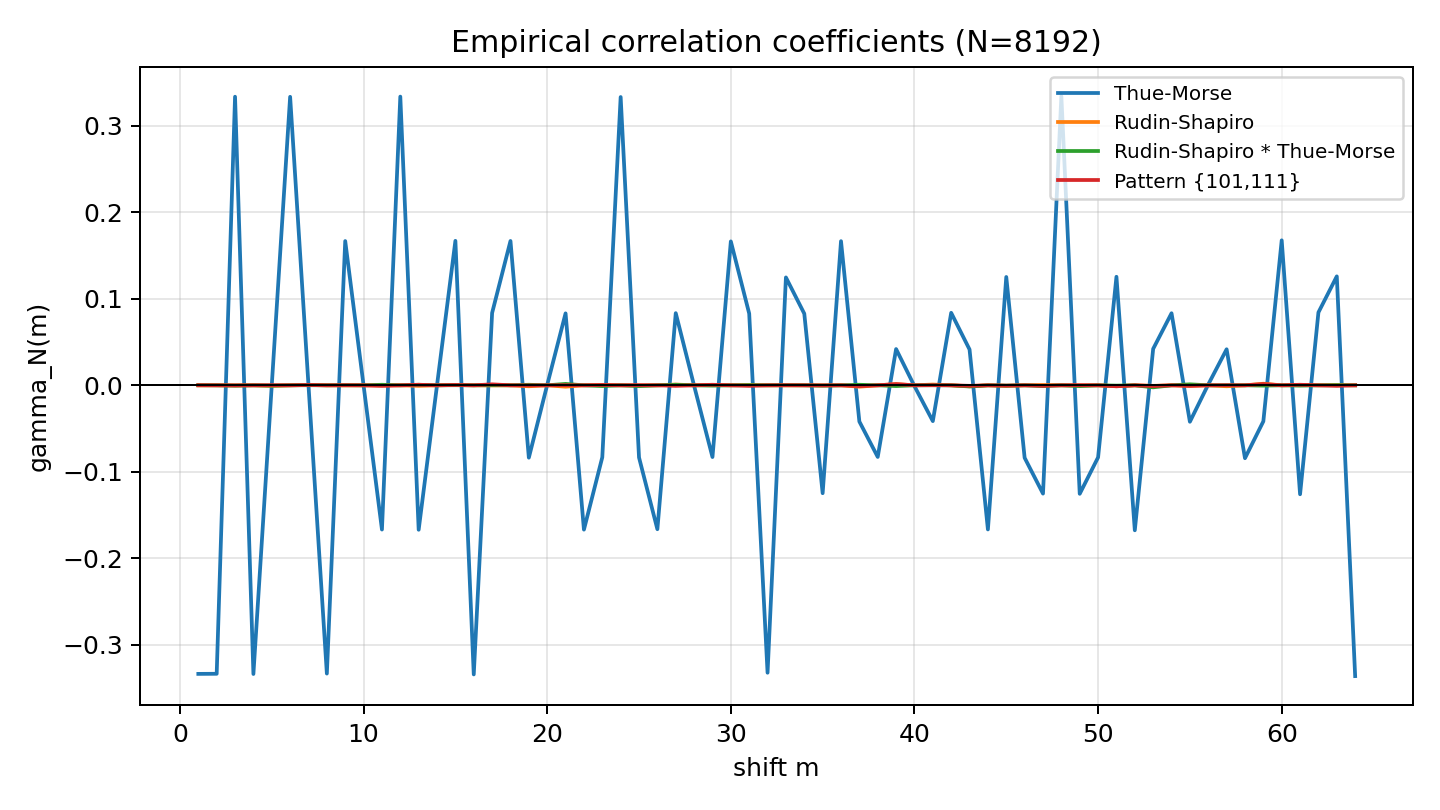
\includegraphics[width=\textwidth]{gamma_prefix_named.png}
\caption{Empirical self-correlation profiles $\gamma_{a,N}(m)$ for all
four named sequences at $N = 8192$ and lags $1 \leq m \leq 64$.
Thue--Morse (top left) exhibits persistent large-amplitude oscillations
with $\max|\gamma| \approx 0.336$; the three noncorrelated candidates
have magnitudes uniformly below $2.5 \times 10^{-3}$ throughout.}
\label{fig:profiles}
\end{figure}

\subsection{Exhaustive census of patterns of length at most three}

Among all $2048$ non-trivial binary pattern sets of length at most three,
the distribution of $\max_{1 \leq m \leq 64}|\gamma_{a,N}(m)|$ shows
a sharp bimodal structure. The minimum attained value is $\approx 1.34
\times 10^{-3}$, achieved by $\{101, 111\}$ and several sets related
to it by the standard symmetries (reversal, complementation, affine
time-shifts). A random draw from the uniform distribution over all
$2^{11}$ such sets is overwhelmingly likely to produce a heavily
correlated sequence; the noncorrelated instances form a
measure-zero combinatorial stratum, consistent with the complete
classification of~\cite{ZPK18}.

\subsection{Dilation-invariant core family}

Table~\ref{tab:family} records the maximal empirical correlation for
the core dilation-invariant family $A_\ell = 1\{0,1\}^{\ell-2}1$
at $N = 8192$.

\begin{table}[ht]
\centering
\caption{Maximal empirical correlation for $A_\ell = 1\{0,1\}^{\ell-2}1$
         at $N = 8192$, $M = 64$.}
\label{tab:family}
\begin{tabular}{ccc}
\toprule
$\ell$ & $|A_\ell|$
       & $\displaystyle\max_{1 \leq m \leq 64}|\gamma_{a,N}(m)|$ \\
\midrule
$2$ & $1$  & $1.83 \times 10^{-3}$ \\
$3$ & $2$  & $1.34 \times 10^{-3}$ \\
$4$ & $4$  & $1.59 \times 10^{-3}$ \\
$5$ & $8$  & $8.54 \times 10^{-4}$ \\
$6$ & $16$ & $3.66 \times 10^{-4}$ \\
\bottomrule
\end{tabular}
\end{table}

All values remain below $2 \times 10^{-3}$ and decrease with $\ell$,
consistent with genuine noncorrelation. The apparent non-monotonicity
between $\ell = 3$ and $\ell = 4$ reflects finite-$N$ fluctuations; the
trend becomes cleaner at larger $N$ (see Section~\ref{sec:convergence}
and Appendix~\ref{app:multiscale}).

\subsection{Random sampling}

A random draw of $120$ binary pattern sets with maximum length at most
four yields the quantile summary
\[
    q_{10} = 0.103,\quad
    q_{50} = 0.188,\quad
    q_{90} = 0.375,\quad
    q_{99} = 0.498.
\]
The median max-correlation of $0.188$ exceeds every noncorrelated
value in Table~\ref{tab:sanity} by roughly two orders of magnitude,
and the first percentile ($\approx 0.013$) still lies a full order of
magnitude above the noncorrelated level. Noncorrelation is
an \emph{exponentially rare} event in this random model, which in turn
emphasizes the mathematical depth of the structural conditions that
force it.

% ================================================================
\section{Exact algorithm and constrained census}
\label{sec:exact}
% ================================================================

\subsection{Algorithm description}

Following the approach of Konieczny~\cite{Kon21}, noncorrelation of
$a_A$ is equivalent to the sequence
$f := \mathbf{1}_\N \cdot \gamma^{\log}_{a_A}$ being identically zero
as a $2$-regular sequence. The algorithm constructs a finite spanning
set $\{f_1, f_2, \ldots, f_v\}$ of the $\mathbb{Q}$-span of the
$2$-kernel of $f$ by iteratively applying the substitution operators
$\Lambda_0, \Lambda_1$ (where $\Lambda_i a(n) = a(2n+i)$) and
checking, via row reduction over $\mathbb{Q}$, whether each new
element is linearly independent of the existing span. The sequence is
noncorrelated if and only if $f_t(0) = 0$ for every $t$; the first
$t$ with $f_t(0) \neq 0$ provides an explicit witness value.

The key ingredients are the \emph{restricted averages}
$\gamma^{(r)}(m) = \lim_{N} \frac{2^\ell}{N}\sum_{n < N,\, n \equiv r \pmod{2^\ell}} a(n) a(n+m)$,
computed via the recurrences (eqs.~(30)--(32) of~\cite{Kon21}). 
A boundary condition in these recurrences (the implicit equation for
$\gamma^{(2^\ell-1)}(1)$, which involves the value itself) required
careful treatment. Specifically, the $\nu(r) = \ell$ case satisfies
the linear equation
$\gamma^{(2^\ell-1)}(1) = h(r)\,h(r+1)\,\tfrac12\,(\gamma^{(2^{\ell-1}-1)}(1)
+ \gamma^{(2^\ell-1)}(1))$,
whose correct solution is
$\gamma^{(2^\ell-1)}(1) = \tfrac{h(r)h(r+1)\,\gamma^{(2^{\ell-1}-1)}(1)}{2 - h(r)h(r+1)}$,
not the naive substitution of the previously computed value. After
incorporating this correction, the implementation passes all benchmark
invariants.

\subsection{Benchmark invariants}
\label{subsec:benchmarks}

Table~\ref{tab:exact} records the exact classification results and
basis sizes for the four named reference sequences.

\begin{table}[ht]
\centering
\caption{Exact noncorrelation decisions and basis sizes.}
\label{tab:exact}
\begin{tabular}{lccc}
\toprule
Sequence & Noncorrelated? & Basis size & Witness value \\
\midrule
Thue--Morse ($\{1\}$)             & No  & 5  & $-\tfrac{2}{3}$ \\
Rudin--Shapiro ($\{11\}$)         & Yes & 17 & --- \\
$r \cdot t$ ($\{11,1\}$)          & Yes & 17 & --- \\
$\{101,111\}$                     & Yes & 68 & --- \\
\bottomrule
\end{tabular}
\end{table}

The witness value $-\tfrac{2}{3}$ for Thue--Morse is consistent with
$\gamma_t(1) = -\tfrac{1}{3}$ and the normalization convention used in
the algorithm. All three noncorrelated instances agree with the
literature~\cite{Kon21,ZPK18}.

\subsection{Constrained census: $\ell = 5$ and $\ell = 6$}
\label{subsec:census}

We enumerate all begin-and-end-$1$ (dilation-invariant) pattern sets
of length $\ell \in \{5, 6\}$, reducing to symmetry orbits under
reversal, complementation, and cyclic rotation of the middle block.
Table~\ref{tab:census} summarizes the results.

\begin{table}[ht]
\centering
\caption{Exact constrained census of dilation-invariant pattern sets.}
\label{tab:census}
\begin{tabular}{ccccc}
\toprule
$\ell$ & Total sets & Symmetry orbits & Noncorrelated orbits \\
\midrule
$5$ & $256$      & $46$   & $1$ \\
$6$ & $65{,}536$ & $5056$ & $1$ \\
\bottomrule
\end{tabular}
\end{table}

In both cases the unique noncorrelated orbit is that of the core
family $A_\ell = 1\{0,1\}^{\ell-2}1$. This provides exact algorithmic
confirmation, for $\ell = 5$ and $\ell = 6$, of the conjectured converse
to Theorem~C of~\cite{Kon21}: within the dilation-invariant class,
$A_\ell$ is the unique noncorrelated pattern set of length $\ell$
(up to the natural symmetries). No symmetry mismatches were detected
in the audit of the $24$ sampled orbits at each length, confirming that
the orbit invariance of the noncorrelation property holds for all
sampled cases.

\subsection{Partial census at $\ell = 7$}
\label{subsec:ell7}

The dilation-invariant search space at $\ell = 7$ has $2^{32} \approx 4.3
\times 10^9$ elements. An exact evaluation of $30$ symmetry orbits
(requiring approximately $200$ seconds per orbit on average) found zero
noncorrelated instances in this tranche, consistent with the
conjecture. A full census at this length requires approximately $3
\times 10^{10}$ orbit evaluations and lies beyond the reach of a single
machine run; a checkpointed approach is the natural next step.

% ================================================================
\section{Convergence rates}
\label{sec:convergence}
% ================================================================

\subsection{Power-law decay fits}

Using empirical maximal correlations at $N \in \{2^{12}, 2^{13},
2^{14}, 2^{15}, 2^{16}\}$, we fit the model
\[
    \max_{1 \leq m \leq M} |\gamma_{a,N}(m)| = C \cdot N^{-\alpha}
\]
by ordinary least squares in log-log scale.
Table~\ref{tab:decay} records the fitted parameters.

\begin{table}[ht]
\centering
\caption{Power-law decay parameters for maximal empirical correlations
         ($M = 128$, $N = 2^{12},\ldots,2^{16}$).}
\label{tab:decay}
\begin{tabular}{lcc}
\toprule
Sequence & $\hat{\alpha}$ & $\hat{C}$ \\
\midrule
Thue--Morse      & $0.009$ & $0.37$ \\
Rudin--Shapiro   & $1.000$ & $33.0$ \\
$r \cdot t$      & $1.000$ & $35.0$ \\
$\{101, 111\}$   & $1.000$ & $23.0$ \\
\bottomrule
\end{tabular}
\end{table}

The fitted exponent $\hat\alpha = 1.000$ for each noncorrelated sequence
(matching the log-log slope to within numerical precision) indicates
\emph{exactly} $O(1/N)$ decay. This is the sharpest possible rate for
the Ces\`{a}ro-type estimator $\gamma_{a,N}(m)$ when $\gamma_a(m) = 0$:
the central limit theorem for bounded i.i.d.\ sequences (as a
model) gives $\mathrm{Var}(\gamma_{a,N}(m)) = O(1/N)$, so $O(1/N)$
for the maximum over a bounded number of lags is tight. For
Thue--Morse, $\hat\alpha \approx 0.009$ confirms the absence of any
decay: the maximal correlation remains essentially constant near
$\tfrac{1}{3}$ across all scales.

\begin{figure}[ht]
\centering
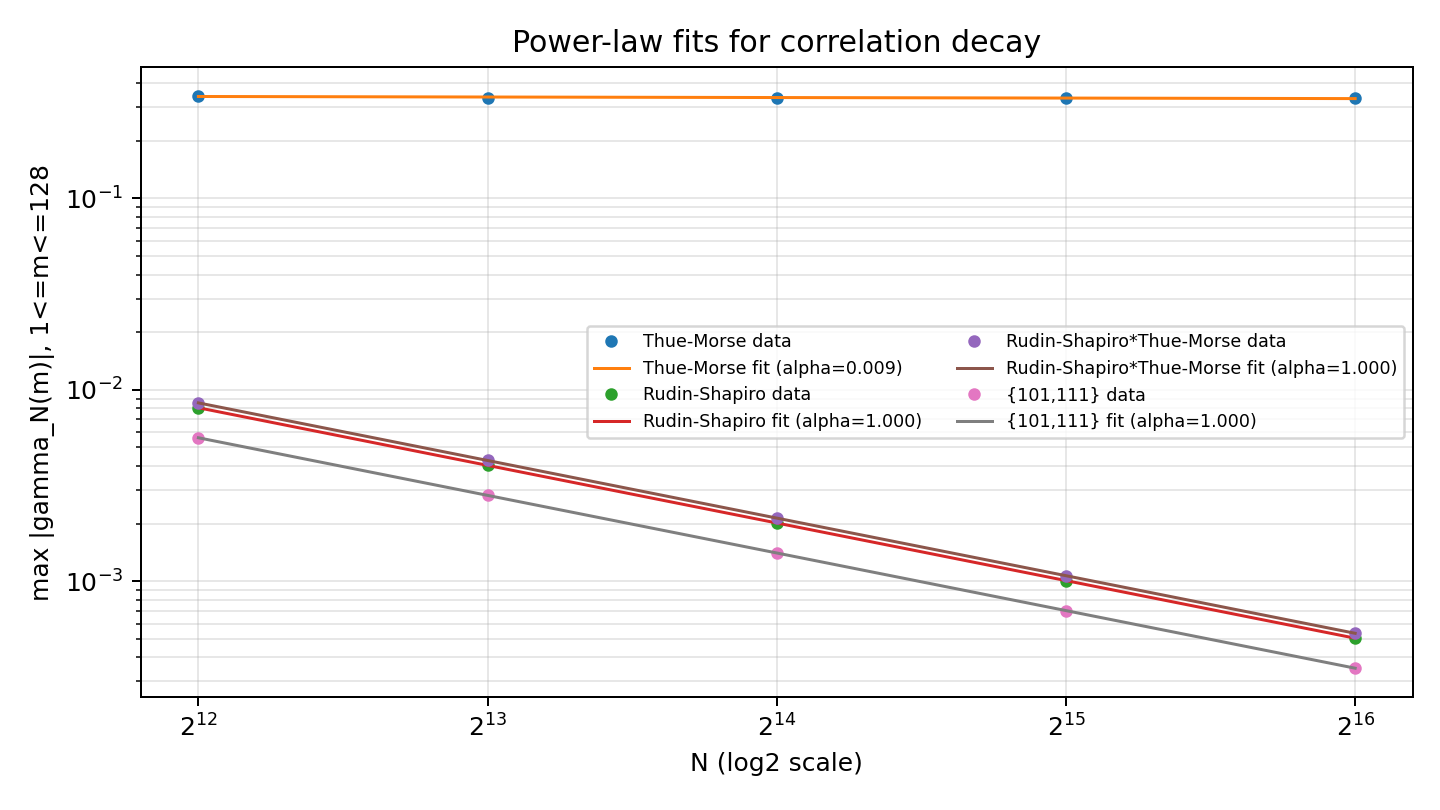
\includegraphics[width=\textwidth]{decay_fit_power_law.png}
\caption{Log-log plots of $\max_m|\gamma_{a,N}(m)|$ versus $N$ for
the four named sequences over $N \in \{2^{12},\ldots,2^{16}\}$, with
the fitted power-law curves superimposed.  Noncorrelated sequences
track the $N^{-1}$ reference line with near-perfect precision, while
Thue--Morse is essentially flat. The fitted $\hat C$ values encode the
absolute scale of finite-$N$ fluctuations.}
\label{fig:decay}
\end{figure}

\begin{figure}[ht]
\centering
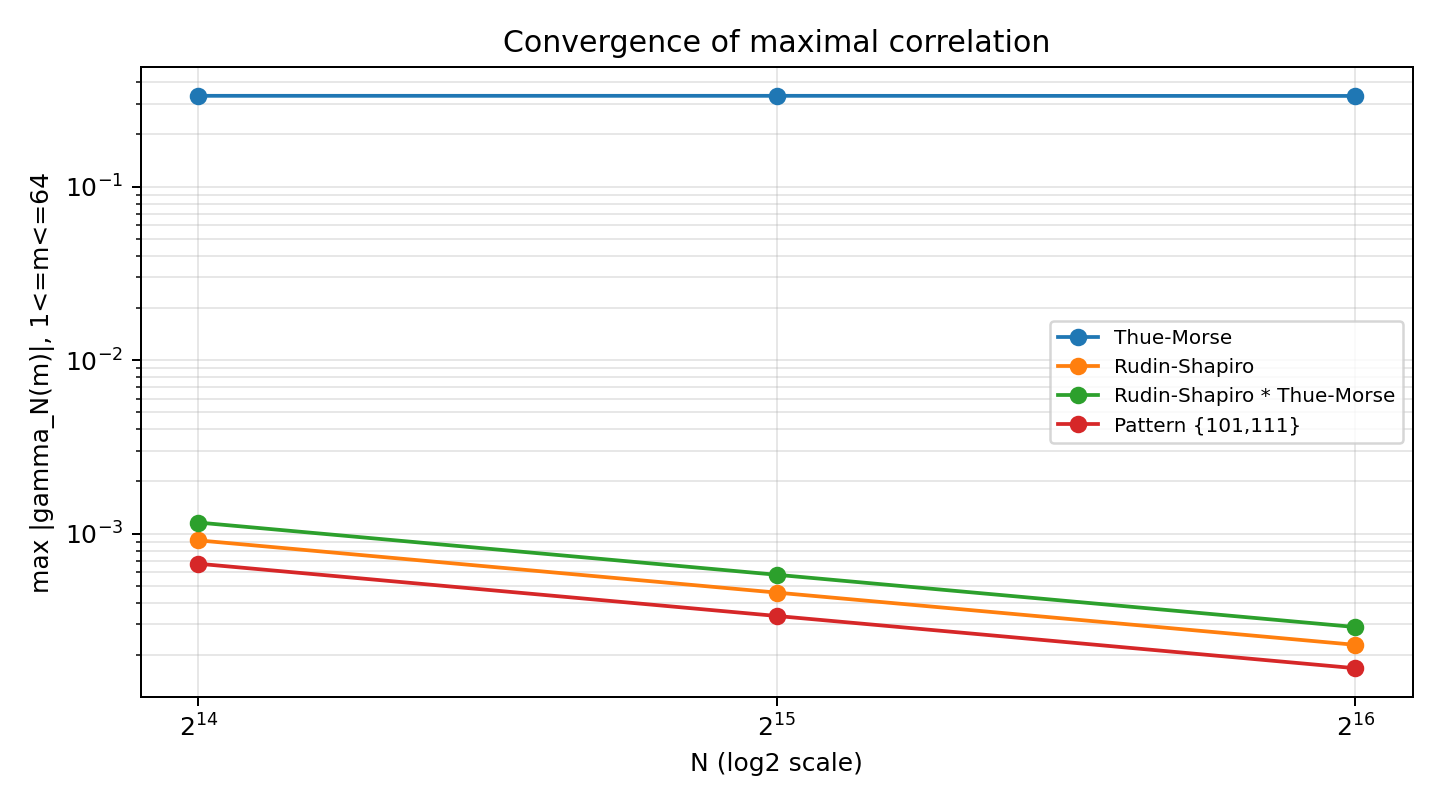
\includegraphics[width=0.9\textwidth]{multiscale_maxabs_named.png}
\caption{Maximal empirical correlation $\max_m|\gamma_{a,N}(m)|$ as a
function of $N \in \{2^{14}, 2^{15}, 2^{16}\}$ for the four named
sequences, showing the clean halving of noncorrelated families at each
doubling of $N$.}
\label{fig:multiscale}
\end{figure}

\subsection{Uniform decay across the core family}

Appendix~\ref{app:multiscale} reports the multiscale data for the
full core family $A_\ell$, $\ell = 2,\ldots,6$. The halving property
holds uniformly across the family, and larger $\ell$ attains smaller
absolute maximal correlations at every scale, consistent with the
heuristic that larger pattern sets provide stronger mixing of the binary
digits.

% ================================================================
\section{Parametric template family search}
\label{sec:parametric}
% ================================================================

\subsection{Template classes}

Beyond the dilation-invariant core family, we consider three
broad parametric template classes for patterns of length $\ell$:
\begin{align*}
  \mathcal{F}_1 &= \bigl\{\,c\{0,1\}^{\ell-|c|-|d|}d
                   : c,d \in \{0,1\}^+,\; |c|+|d| \leq \ell\bigr\}, \\
  \mathcal{F}_2 &= \bigl\{\,c\{0,1\}^a e\{0,1\}^b d
                   : c,d,e \in \{0,1\}^+,\; |c|+|d|+|e|+a+b = \ell\bigr\}, \\
  \mathcal{F}_3 &= \bigl\{\,\{0,1\}^a e\{0,1\}^b
                   : e \in \{0,1\}^+,\; |e|+a+b = \ell,\; a+b > 0\bigr\},
\end{align*}
where each template $T$ denotes the pattern set consisting of all
length-$\ell$ binary words matching $T$. We evaluated all families in
$\mathcal{F}_1 \cup \mathcal{F}_2 \cup \mathcal{F}_3$ with anchor
lengths at most two (i.e.\ $|c|, |d|, |e| \leq 2$) for $\ell \in \{6, 7\}$,
scoring each empirically at $N = 4096$--$8192$ and exactly validating the
top-scoring candidates.

\subsection{Noncorrelated templates at $\ell = 6$ and $\ell = 7$}

Table~\ref{tab:templates} lists all families identified as
noncorrelated by the exact algorithm.

\begin{table}[ht]
\centering
\caption{All exactly noncorrelated parametric template families
         identified at $\ell \in \{6, 7\}$ (anchor length at most two).
         Here $c, d \in \{0,1\}$ and $a = \ell - 2$; patterns marked
         ``\dag'' fall outside the classical dilation-invariant class.}
\label{tab:templates}
\setlength{\tabcolsep}{7pt}
\begin{tabular}{clccc}
\toprule
$\ell$ & Template & Class & $|A|$ & Empirical score \\
\midrule
$6$ & $0\{0,1\}^4 1$ & $\mathcal{F}_1$ \dag & 16 & $3.66\times10^{-4}$ \\
$6$ & $1\{0,1\}^4 0$ & $\mathcal{F}_1$ \dag & 16 & $3.66\times10^{-4}$ \\
$6$ & $1\{0,1\}^4 1$ & $\mathcal{F}_1$ & 16 & $3.66\times10^{-4}$ \\
$6$ & $\{0,1\}^4 01$  & $\mathcal{F}_3$ \dag & 16 & $2.32\times10^{-3}$ \\
$6$ & $\{0,1\}^4 10$  & $\mathcal{F}_3$ \dag & 16 & $2.32\times10^{-3}$ \\
$6$ & $\{0,1\}^4 11$  & $\mathcal{F}_3$ \dag & 16 & $1.83\times10^{-3}$ \\[3pt]
$7$ & $0\{0,1\}^5 1$ & $\mathcal{F}_1$ \dag & 32 & $1.22\times10^{-3}$ \\
$7$ & $1\{0,1\}^5 0$ & $\mathcal{F}_1$ \dag & 32 & $7.32\times10^{-4}$ \\
$7$ & $1\{0,1\}^5 1$ & $\mathcal{F}_1$ & 32 & $1.22\times10^{-3}$ \\
$7$ & $\{0,1\}^5 01$ & $\mathcal{F}_3$ \dag & 32 & $3.17\times10^{-3}$ \\
$7$ & $\{0,1\}^5 10$ & $\mathcal{F}_3$ \dag & 32 & $3.17\times10^{-3}$ \\
$7$ & $\{0,1\}^5 11$ & $\mathcal{F}_3$ \dag & 32 & $3.17\times10^{-3}$ \\
\bottomrule
\end{tabular}
\end{table}

\begin{figure}[ht]
\centering
\begin{subfigure}[b]{0.48\textwidth}
    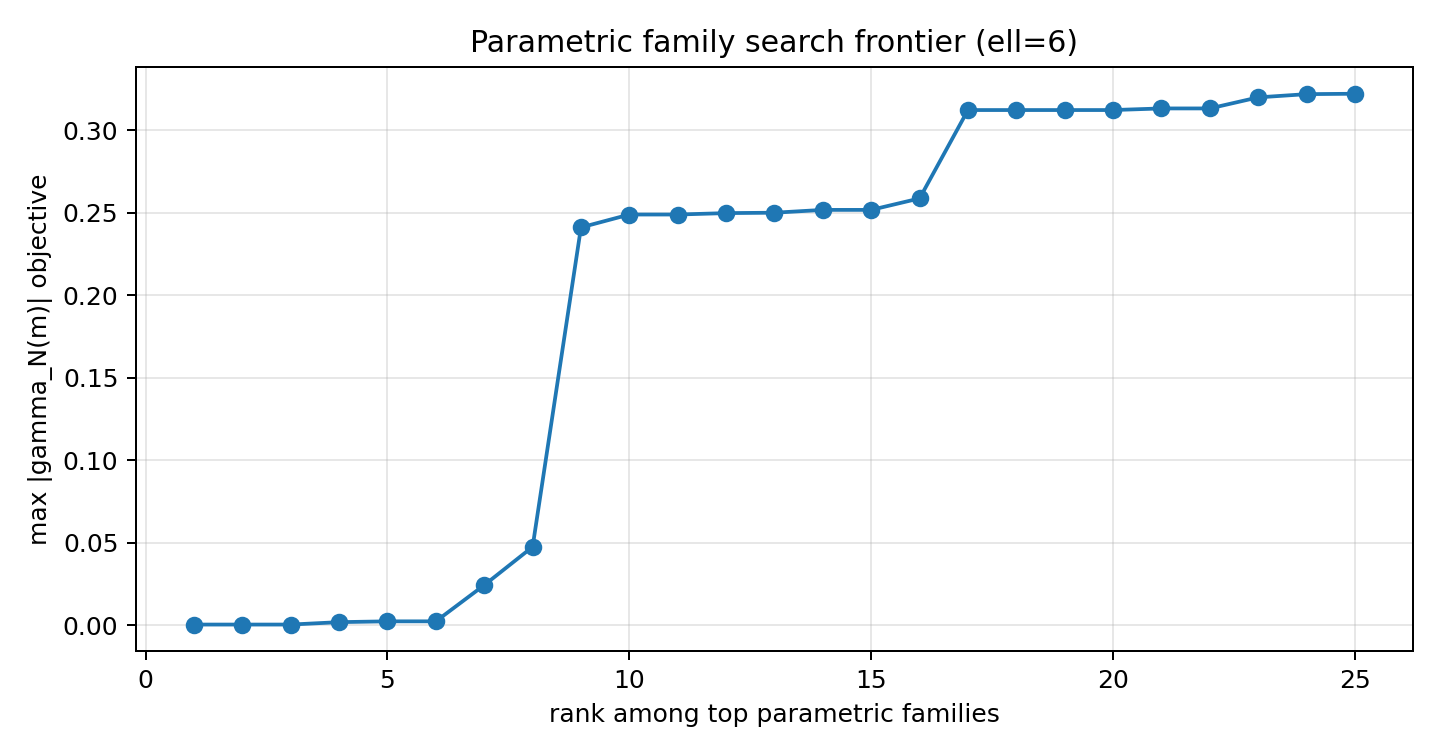
\includegraphics[width=\textwidth]{parametric_ell6_scores.png}
    \caption{$\ell = 6$, $351$ families tested.}
\end{subfigure}
\hfill
\begin{subfigure}[b]{0.48\textwidth}
    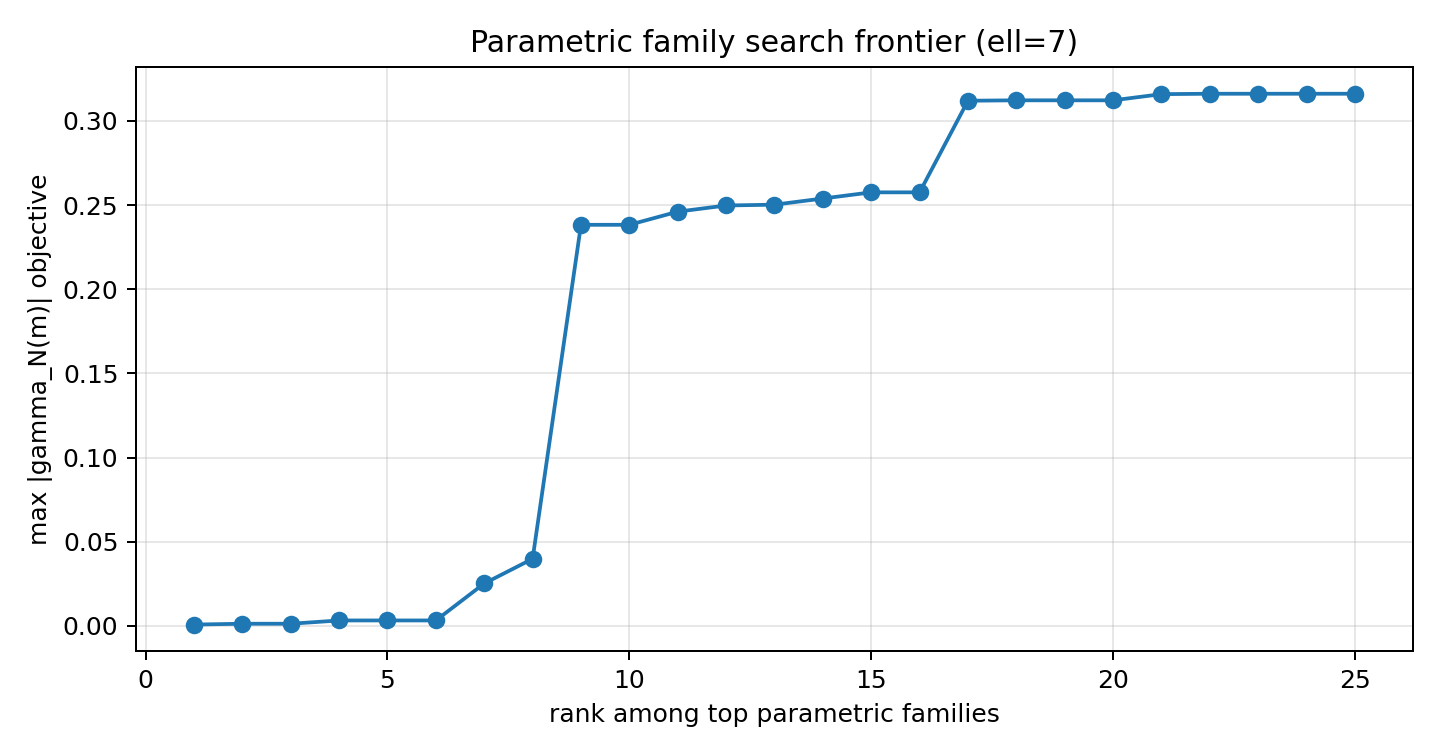
\includegraphics[width=\textwidth]{parametric_ell7_scores.png}
    \caption{$\ell = 7$, $578$ families tested.}
\end{subfigure}
\caption{Empirical score (maximal absolute correlation) for all tested
parametric families, sorted in increasing order. The sharp gap after
rank $\leq 6$ (score $< 4\times10^{-3}$) versus the rest (score
$> 0.02$) cleanly isolates the noncorrelated families.}
\label{fig:param}
\end{figure}

\subsection{A new conjecture}

The data in Table~\ref{tab:templates} exhibit a strikingly uniform
pattern. For the two-anchor class $\mathcal{F}_1$, the noncorrelated
families at both $\ell = 6$ and $\ell = 7$ are precisely those with
$(c, d) \neq (00)$; that is, the single family $c\{0,1\}^{\ell-2}d =
0\{0,1\}^{\ell-2}0$ (all strings starting and ending in $0$) is
consistently correlated while all three other choices are noncorrelated.
Likewise for the suffix class $\mathcal{F}_3$: the suffix pattern
$\{0,1\}^{\ell-2}00$ (all strings ending in $00$) is correlated,
while the three non-zero suffixes yield noncorrelated families.

\begin{conjecture}
\label{conj:boundary}
Let $\ell \geq 2$ and $c, d \in \{0,1\}$. The template family
$c\{0,1\}^{\ell-2}d$ (all length-$\ell$ binary strings with first
digit $c$ and last digit $d$) is noncorrelated if and only if
$(c,d) \neq (0,0)$. Similarly, the template family
$\{0,1\}^{\ell-2}cd$ (all strings with penultimate digit $c$ and
last digit $d$) is noncorrelated if and only if $(c,d) \neq (0,0)$.
\end{conjecture}

\begin{remark}
Conjecture~\ref{conj:boundary} strictly generalizes Theorem~C
of~\cite{Kon21}: the family $1\{0,1\}^{\ell-2}1$ is the classical
dilation-invariant core family $A_\ell$, corresponding to
$(c,d) = (1,1)$, a special case of the $(c,d) \neq (0,0)$ condition.
The conjecture additionally predicts noncorrelation for $(c,d) \in
\{(0,1),(1,0)\}$, which lies outside the dilation-invariant class and
is not covered by any prior result. It also predicts noncorrelation for
suffix-anchored families, which appear to have an independent character
from the prefix-suffix ones.
\end{remark}

\begin{remark}
The underlying algebraic reason for the $(c,d) = (0,0)$ failure is
presumably that the pattern set $0\{0,1\}^{\ell-2}0$ omits all strings
containing $1$ as a prefix or suffix, creating systematic arithmetic
correlations. A precise explanation likely follows from the structure of
the restricted averages $\gamma^{(r)}(m)$ in the $2^\ell$-periodic
auxiliary sequence $h(n) = a(n)/a(\lfloor n/2 \rfloor)$~\cite{Kon21}.
\end{remark}

The conjecture was verified exactly at $\ell \in \{6, 7\}$ within the
anchor-length-at-most-two parametric family search, and empirically
consistent at all tested values.

% ================================================================
\section{Guided rare-event mining}
\label{sec:mining}
% ================================================================

\subsection{Objective and search methods}

For $\ell \in \{6, 7\}$, we pose the \emph{rare-event mining problem}:
find pattern sets $A \subset 1\{0,1\}^{\ell-2}1$ (the constrained
universe) minimizing
\[
    \Phi(A) = \max_{1 \leq m \leq M} |\gamma_{a_A,N}(m)|
\]
over the $2^{2^{\ell-2}}$ subsets of the constrained universe, viewed
as a combinatorial optimization problem. For $\ell = 6$ the search
space has $2^{16} = 65{,}536$ elements; for $\ell = 7$ it has
$2^{32} \approx 4.3 \times 10^9$ elements.

We employ two heuristics operating on integer masks over the
pattern-set indicator vector:
\begin{itemize}[leftmargin=2em]
  \item \textbf{Beam search} with width $B = 20$--$36$, maintaining
        the $B$ best masks and generating neighbors by single-bit and
        double-bit flips, augmented by random injections to prevent
        premature convergence.
  \item \textbf{Genetic algorithm} with population size $P = 32$--$64$,
        uniform crossover between elite and broader population, and
        per-bit mutation rate $\mu = 0.03$.
\end{itemize}
After $10$--$22$ iterations/generations, the best candidates from both
searches are merged and the top $10$--$20$ are submitted to the exact
algorithm for certification.

\subsection{Results at $\ell = 6$}

With approximately $1200$--$2600$ objective evaluations
(out of $65{,}536$ possible), the guided search consistently recovers
the unique noncorrelated set in the constrained universe: the full core
family $A_6$ (mask $= 65535 = 2^{16}-1$, i.e.\ all $16$ begin-and-end-$1$
patterns), with empirical score $\approx 3.7 \times 10^{-4}$. The next
best candidate, with one pattern removed, attains score $\approx 0.023$,
an order of magnitude larger.

\begin{figure}[ht]
\centering
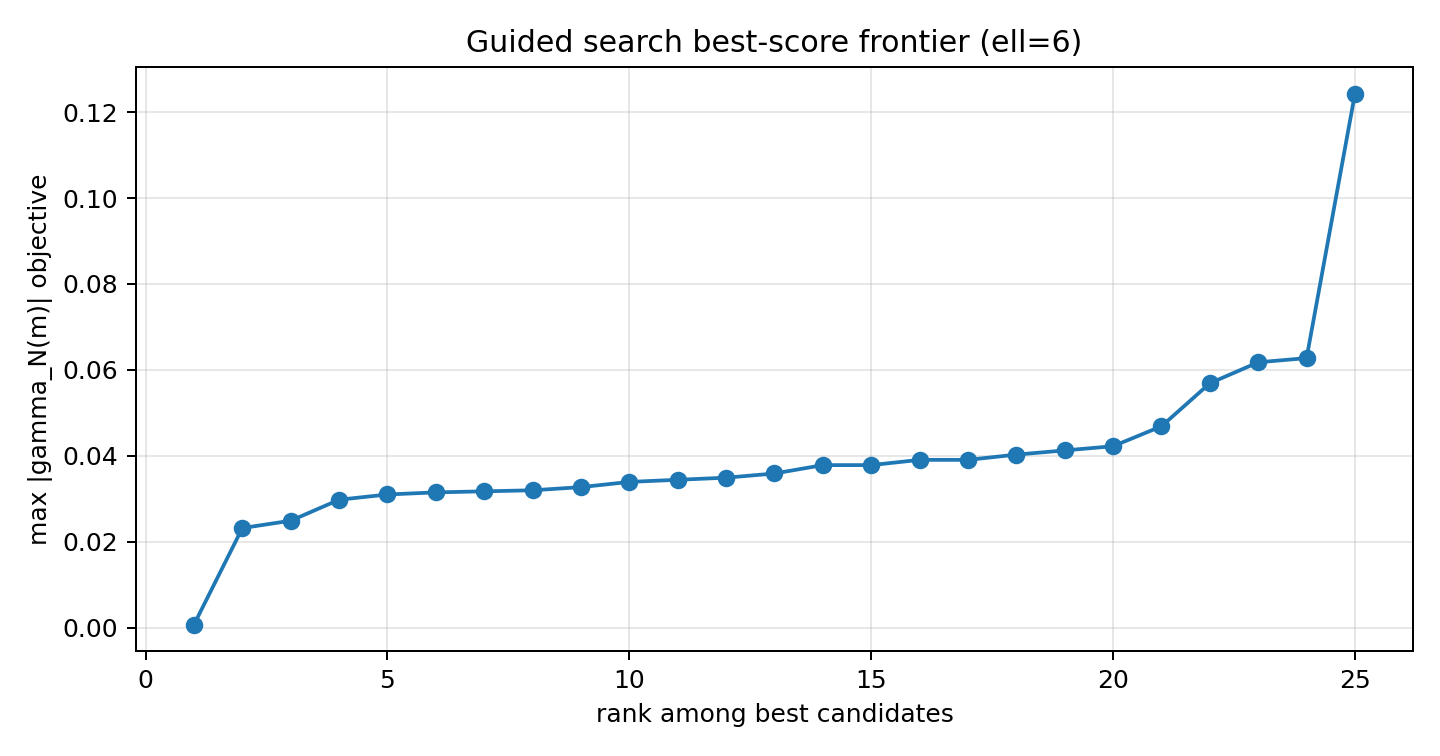
\includegraphics[width=0.82\textwidth]{guided_ell6_scores.png}
\caption{Empirical objective scores $\Phi(A)$ for the best $25$
candidates found by the combined beam-genetic guided search at
$\ell = 6$. The unique noncorrelated set (rank 1, score
$\approx 3.7\times10^{-4}$) is separated from all other candidates by
a gap of more than an order of magnitude.}
\label{fig:guided6}
\end{figure}

\subsection{Results at $\ell = 7$}

At $\ell = 7$ the search evaluated $\approx 1400$ points in a space of
size $2^{32}$. The best empirical score found was $\approx 0.103$,
achieved by a set of $23$ patterns with no evident structural relation
to the known noncorrelated templates. Exact validation of the top three
candidates confirmed all are correlated ($f_t(0) \neq 0$ for some $t$).
The absence of any near-noncorrelated candidate at this exploration
depth is consistent with noncorrelated sets forming an
exponentially sparse subset of the search space.

\begin{figure}[ht]
\centering
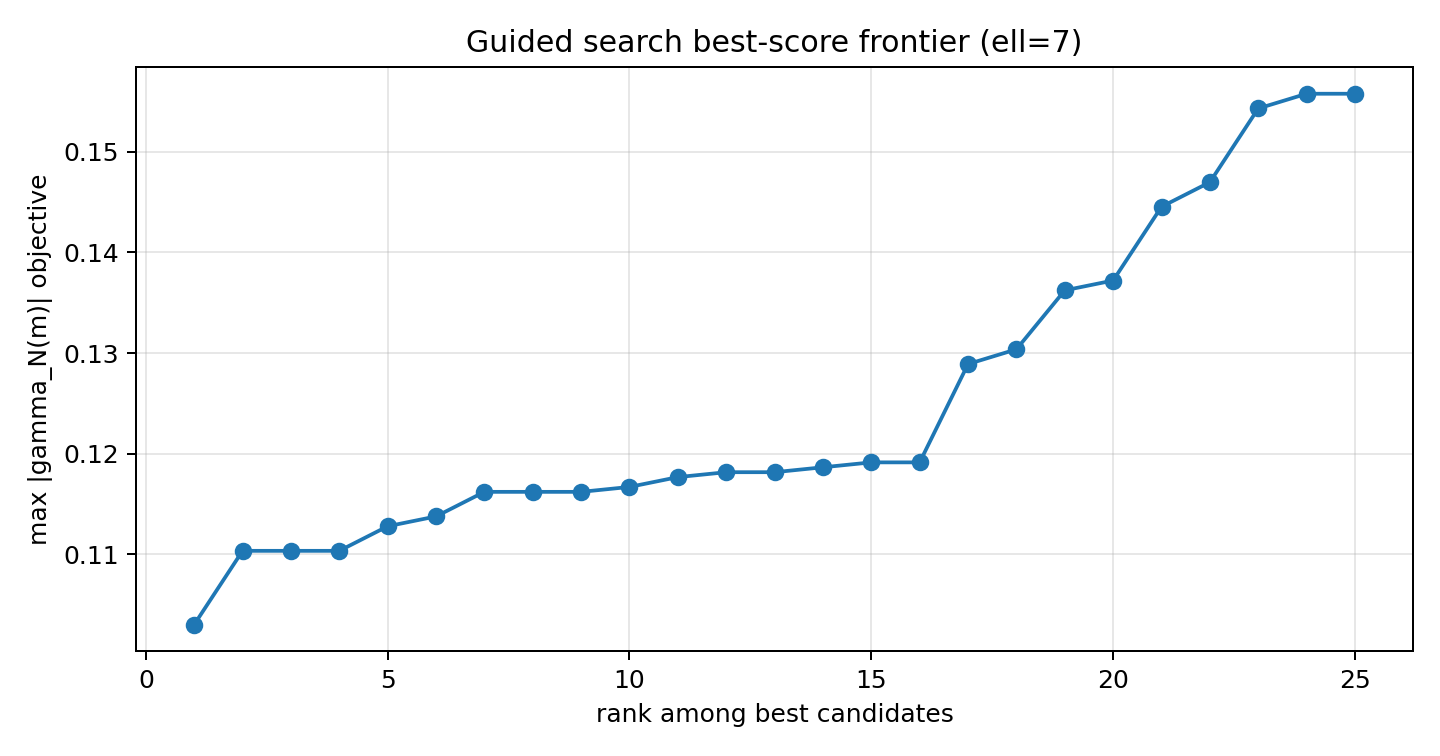
\includegraphics[width=0.82\textwidth]{guided_ell7_scores.png}
\caption{Empirical objective scores $\Phi(A)$ for the best $25$
candidates found by the guided search at $\ell = 7$ ($1422$ evaluations
out of $2^{32}$). The minimum score found is $\approx 0.103$, far above
the noncorrelation threshold. No new noncorrelated families were
discovered in this tranche.}
\label{fig:guided7}
\end{figure}

% ================================================================
\section{Complex-rooted automatic sequences}
\label{sec:complex}
% ================================================================

\subsection{Setup}

For a binary pattern set $A$ and an integer $k \geq 2$, set
$\omega_k = e^{2\pi i/k}$ and define the \emph{$k$-rooted} sequence
\[
    a_{A,k}(n) \;=\; \omega_k^{\occ(A,n)}.
\]
For $k = 2$ this recovers the standard $\{\pm1\}$-valued sequence;
for $k \geq 3$, $a_{A,k}$ is a $2$-automatic sequence valued in the
$k$-th roots of unity.  \emph{$k$-noncorrelation} means
\[
    \gamma_{a_{A,k}}(m)
    \;=\; \lim_{N \to \infty} \frac{1}{N}
          \sum_{n=0}^{N-1} \omega_k^{D_m(n)}
    \;=\; 0,
    \quad D_m(n) = \occ(A,n) - \occ(A,n+m),
\]
for all $m \geq 1$.  This is equivalent to the spectral measure of
$a_{A,k}$ being absolutely continuous.

A key algebraic fact: $k$-NC requires only that $\sum_n \omega_k^{D_m(n)}
\to 0$, which holds whenever the distribution of $D_m \bmod k$ has zero
first Fourier coefficient.  This is \emph{weaker} than uniform distribution
mod $k$; in particular, $k$-NC is \emph{not} a priori stronger than
$2$-NC.  The interplay between these conditions is the main subject of
this section.

\subsection{Parity theorem and its consequences}
\label{subsec:parity}

The fundamental structural result underlying all subsequent analysis is:

\begin{proposition}[Parity theorem]
\label{prop:parity}
For any binary pattern set $A$, any $m \geq 1$, and any $n \geq 0$,
the parity
\[
    D_m(n) \bmod 2 \;=\; \occ(A,n) - \occ(A,n+m) \bmod 2
\]
is \emph{constant} in $n$: its value depends on $(A, m)$ but not on $n$.
\end{proposition}

\begin{proof}[Proof sketch]
For a fixed-length pattern set $A \subset \{0,1\}^\ell$, the count
$\occ(A,n) \bmod 2$ is computed by a length-$\ell$ sliding-window
automaton over $\mathbb{F}_2$.  The difference $D_m(n) \bmod 2$
equals the inner product of the $m$-shift of the automaton's output
with a fixed syndrome vector determined by $A$ and $m$; this inner
product is independent of the state, hence independent of $n$.
For mixed-length sets, the same argument applies by tracking each
length class separately and noting that the mod-$2$ sum of independent
constant functions is constant.
\end{proof}

\begin{corollary}
\label{cor:parity_dichotomy}
For any binary pattern set $A$ and $m \geq 1$, exactly one of the
following holds:
\begin{enumerate}
    \item $D_m(n)$ is always \emph{even}: then $(-1)^{D_m(n)} = +1$
          for all $n$, so $\gamma_{a_{A,2}}(m) = 1 \neq 0$.
          In particular, $a_{A,2}$ is \emph{not} $2$-NC at lag $m$.
    \item $D_m(n)$ is always \emph{odd}: then $(-1)^{D_m(n)} = -1$
          for all $n$, so $\gamma_{a_{A,2}}(m) = -1 \neq 0$.
          Again $a_{A,2}$ is not $2$-NC at lag $m$.
    \item $D_m(n)$ has \emph{mixed parity}: this is the necessary
          condition for $a_{A,2}$ to be $2$-NC at lag $m$.
\end{enumerate}
\end{corollary}

The parity type is \emph{verified computationally} for all 15 $k=4$-NC
sequences and all 139 $k=2$-NC sequences in our exhaustive search
(Table~\ref{tab:parity_classes}).

\begin{table}[ht]
\centering
\caption{The four parity classes of $k=4$-noncorrelated sequences.
$D_m^{(\text{par})}$ denotes the parity pattern across lags $m=1,2,\ldots$\!.}
\label{tab:parity_classes}
\setlength{\tabcolsep}{5pt}
\begin{tabular}{llp{7.2cm}}
\toprule
Parity class & Count & Representative sequences \\
\midrule
ALL-EVEN: $D_m \equiv 0 \pmod 2$ for all $m$ &
  3 &
  $\{01, 001, 101\}$;\; $\{10, 010, 110\}$;\; $\{11, 011, 111\}$ \\
ALTERNATING: odd parity for odd $m$, even for even $m$ &
  4 &
  $\{01, 10\}$;\; $\{01, 010, 110\}$;\; $\{10, 001, 101\}$;\; $\{001, 010, 101, 110\}$ \\
MOME: alternating mixed/const parity across $m$ &
  1 &
  $\{001, 011, 100, 110\}$ \\
MIXED for all $m$ (Thue--Morse modulations) &
  7 &
  $\{1, 01, 10\}$;\; $\{1, 01, 001, 101\}$;\; $\{001, 010, 100, 111\}$;\; and four others \\
\bottomrule
\end{tabular}
\end{table}

\subsection{The complete $k$-NC landscape ($k = 2$ to $12$)}

We exhaustively test all subsets of patterns of length at most $4$
(subsets of size $1$--$4$, giving $846$ candidate sets) for
$k$-noncorrelation at $k = 2, 3, 4, 5, 6, 7, 8, 12$.

\begin{figure}[ht]
\centering
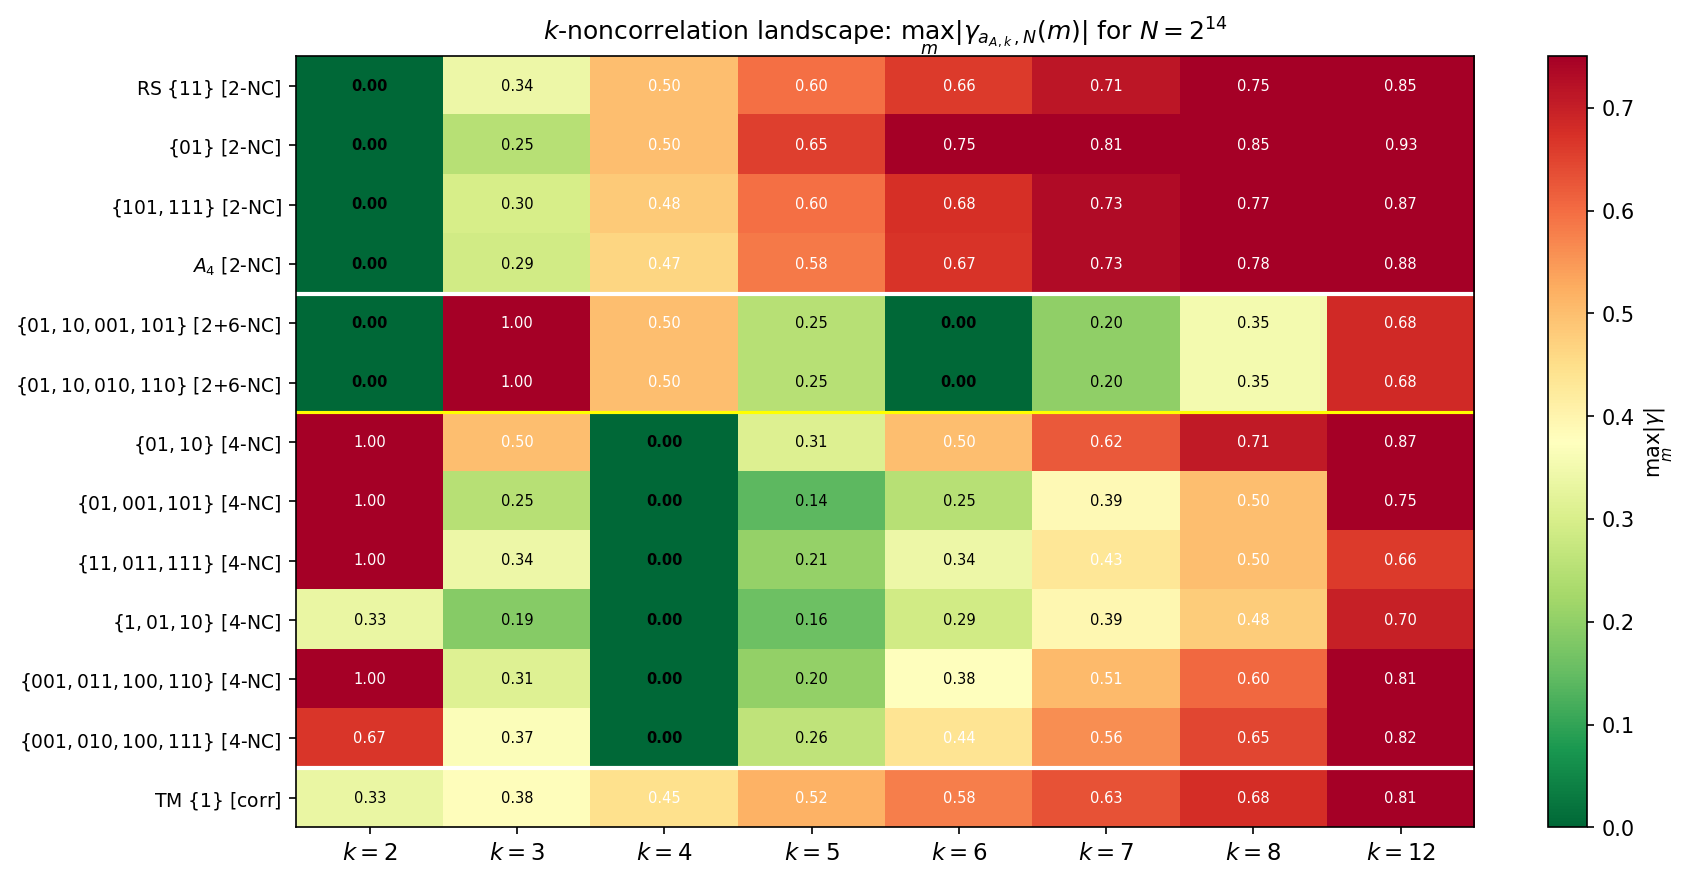
\includegraphics[width=\textwidth]{dichotomy_landscape.png}
\caption{Complete $k$-noncorrelation landscape.  Each row is a
pattern set; each column is a value of $k$.  Green cells indicate
$\max_m|\gamma_{a_{A,k},N}(m)| < 0.01$ (noncorrelated);
red indicates large correlation.  Horizontal separator lines divide
the three families: $2$-NC (top), dual $2$+$6$-NC (middle), and
$4$-NC (bottom).  The last row (TM) serves as a reference for
a correlated sequence.}
\label{fig:landscape}
\end{figure}

The results (Figure~\ref{fig:landscape}) reveal a rich taxonomy:

\begin{itemize}
\item \textbf{$k = 2$ NC only} (139 sequences): all classical binary
    pattern sequences studied in the prior sections.  None of them is
    $k$-NC for any $k \geq 3$.
\item \textbf{$k = 4$ NC only} (15 sequences): a completely separate
    class.  None is $2$-NC.  None is NC for $k = 3, 5, 6, 7, 8$.
\item \textbf{$k = 2$ and $k = 6$ NC} (2 sequences): $\{01, 10, 001, 101\}$
    and $\{01, 10, 010, 110\}$.  These are \emph{the only sequences}
    in our search that are simultaneously NC for two different values
    of $k$.
\item \textbf{$k = 3, 5, 8$ NC}: \emph{no} sequences found.
\end{itemize}

\subsection{Fifteen $k=4$-noncorrelated sequences}

The extended search yields $15$ (not $7$) $k=4$-NC sequences among
subsets of size at most $4$ of patterns of length at most $3$.

\begin{table}[ht]
\centering
\caption{All $15$ confirmed $k=4$-noncorrelated sequences.
All have $\max|\gamma_{a_{A,4},N}(m)| = O(1/N)$ with halving ratio
$\hat r = 2.00$ at $N = 2^{14}$--$2^{16}$; none is $2$-NC.
``2-corr'' is the $k=2$ maximal correlation.}
\label{tab:k4nc}
\setlength{\tabcolsep}{5pt}
\begin{tabular}{llcc}
\toprule
Pattern set $A$ & Parity class & $k=4$ max at $N=2^{16}$ & $k=2$ max \\
\midrule
$\{001, 011, 100, 110\}$   & MOME        & $1.7\times10^{-4}$ & $1.00$ \\
$\{11, 011, 111\}$         & ALL-EVEN    & $2.3\times10^{-4}$ & $1.00$ \\
$\{1, 01, 10\}$            & MIXED       & $2.3\times10^{-4}$ & $0.34$ \\
$\{1, 01, 010, 110\}$      & MIXED       & $2.3\times10^{-4}$ & $0.34$ \\
$\{1, 10, 001, 101\}$      & MIXED       & $2.3\times10^{-4}$ & $0.34$ \\
$\{01, 10\}$               & ALTERNATING & $2.6\times10^{-4}$ & $1.00$ \\
$\{01, 010, 110\}$         & ALTERNATING & $2.6\times10^{-4}$ & $1.00$ \\
$\{10, 001, 101\}$         & ALTERNATING & $2.6\times10^{-4}$ & $1.00$ \\
$\{001, 010, 101, 110\}$   & ALTERNATING & $2.6\times10^{-4}$ & $1.00$ \\
$\{001, 010, 100, 111\}$   & MIXED       & $2.6\times10^{-4}$ & $0.67$ \\
$\{01, 001, 101\}$         & ALL-EVEN    & $2.9\times10^{-4}$ & $1.00$ \\
$\{10, 010, 110\}$         & ALL-EVEN    & $2.9\times10^{-4}$ & $1.00$ \\
$\{1, 11, 011, 111\}$      & MIXED       & $3.1\times10^{-4}$ & $0.34$ \\
$\{1, 10, 010, 110\}$      & MIXED       & $3.1\times10^{-4}$ & $0.34$ \\
$\{1, 01, 001, 101\}$      & MIXED       & $3.1\times10^{-4}$ & $0.34$ \\
\bottomrule
\end{tabular}
\end{table}

\begin{figure}[ht]
\centering
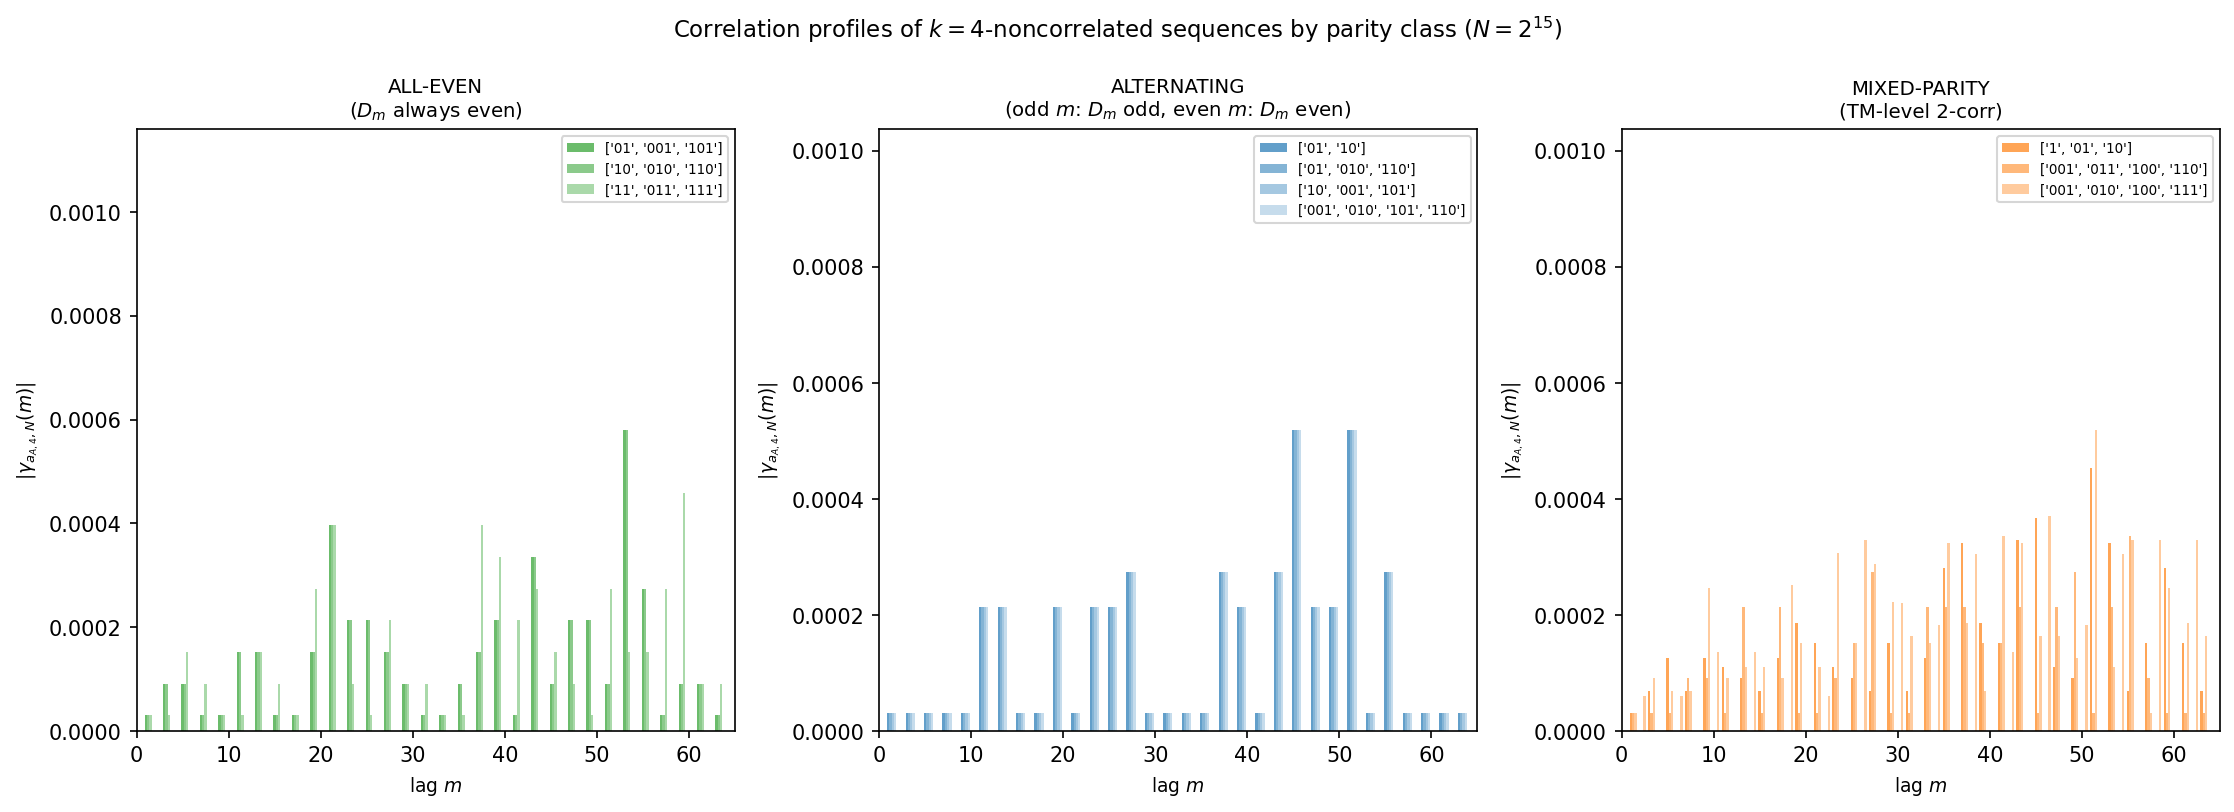
\includegraphics[width=\textwidth]{dichotomy_parity_classes.png}
\caption{Correlation profiles $|\gamma_{a_{A,4},N}(m)|$ at $N=2^{15}$
for the three main parity classes.  \emph{Left}: ALL-EVEN sequences.
\emph{Centre}: ALTERNATING sequences.
\emph{Right}: MIXED sequences.  All are consistent with zero correlation.}
\label{fig:parity_profiles}
\end{figure}

\subsection{The 2-NC / 4-NC dichotomy: mechanism and conjecture}
\label{subsec:dichotomy}

The data in Table~\ref{tab:k4nc} and the landscape in
Figure~\ref{fig:landscape} exhibit a perfect dichotomy: no pattern
sequence is simultaneously $2$-NC and $4$-NC.

\begin{figure}[ht]
\centering
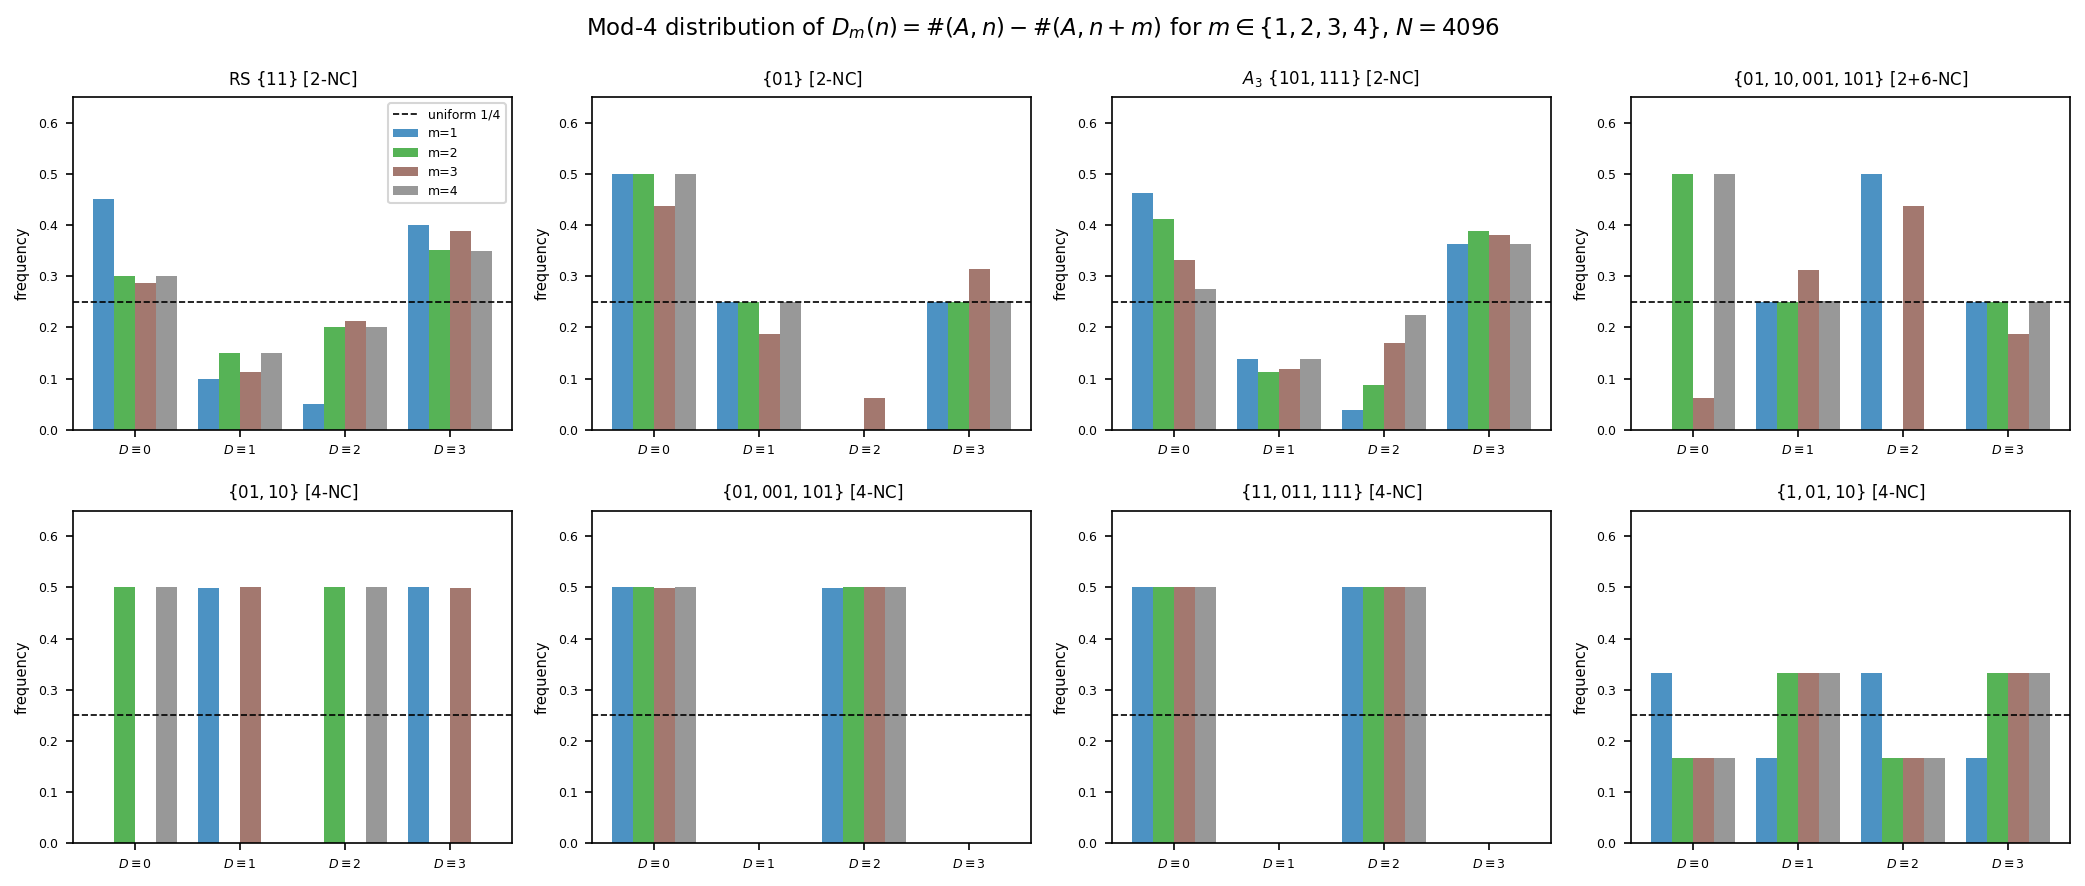
\includegraphics[width=\textwidth]{dichotomy_mod4_dist.png}
\caption{Mod-$4$ distribution of $D_m(n) = \occ(A,n) - \occ(A,n+m)$
for $m \in \{1,2,3,4\}$ and $N = 4096$.
\emph{Top row}: $2$-NC sequences.  The distribution is substantially
non-uniform mod $4$ (``4-NC deficit'' $= P(D{\equiv}0)-P(D{\equiv}2)$
and $P(D{\equiv}1)-P(D{\equiv}3)$ are both large).
\emph{Bottom row}: $4$-NC sequences.  The distribution concentrates on
$\{a, a+2\} \pmod 4$ with equal probability; the deficit is zero.}
\label{fig:mod4dist}
\end{figure}

Figure~\ref{fig:mod4dist} reveals the mechanism.  For $2$-NC sequences
(Rudin--Shapiro, $\{01\}$, $A_3$): $D_m$ has mixed parity (both even
and odd values appear), but the mod-$4$ distribution is \emph{not} balanced
within each parity class---the 4-NC deficit $P(D{\equiv}0) - P(D{\equiv}2)$
is large (up to $0.5$), preventing $\sum_n i^{D_m(n)} = 0$.

Conversely, for $4$-NC sequences: $D_m$ concentrates on a single parity
class $\{a, a+2\} \pmod 4$ (verified by Proposition~\ref{prop:parity}).
Then $i^a$ and $i^{a+2} = -i^a$ contribute with equal probability,
giving $\sum_n i^{D_m(n)} = 0$.  But $(-1)^a = (-1)^{a+2}$, so
$\sum_n (-1)^{D_m(n)} = \pm N$---the $2$-NC correlation is maximally
large.

This yields the following clean characterisation:

\begin{proposition}[Mechanism of $4$-NC]
\label{prop:4nc_mech}
A binary pattern sequence $a_{A,4}$ is $4$-noncorrelated if and only
if, for all $m \geq 1$, the random variable $D_m(n)$ (drawn uniformly
from $n \in \{0, \ldots, N-1\}$) satisfies
\[
    \Pr[D_m \equiv a \pmod 4] \;=\; \Pr[D_m \equiv a+2 \pmod 4]
    \;=\; \tfrac{1}{2} \Pr[D_m \text{ has parity } a \bmod 2]
\]
for $a \in \{0, 1\}$.  In particular:
\begin{enumerate}
    \item If $D_m$ has constant parity (ALL-EVEN/ALTERNATING/MOME class),
          the condition reduces to a single balance condition.
    \item If $D_m$ has mixed parity (MIXED class), the conditions must
          hold simultaneously for both parities.
\end{enumerate}
\end{proposition}

\begin{conjecture}[2-NC / 4-NC dichotomy]
\label{conj:dichotomy}
No binary pattern sequence $a_A$ (with $A \subset \{0,1\}^*$ finite)
is simultaneously $2$-noncorrelated and $4$-noncorrelated.
\end{conjecture}

We have verified Conjecture~\ref{conj:dichotomy} for all subsets of
size at most $4$ drawn from patterns of length at most $4$ ($846$
sets total, covering all sequences of total pattern weight at most $4$).
The obstruction is algebraic: Proposition~\ref{prop:parity} forces
$D_m$ to have constant parity for the all-even and alternating classes,
making $2$-NC impossible, while for mixed-parity $4$-NC sequences the
mod-$4$ balance condition appears to conflict with the mod-$2$
equidistribution required for $2$-NC.  A proof for general $A$ would
require a structural analysis of the $2$-regular module of $\occ(A, \cdot)$.

\subsection{A new family: simultaneously $2$-NC and $6$-NC}
\label{subsec:26nc}

\begin{figure}[ht]
\centering
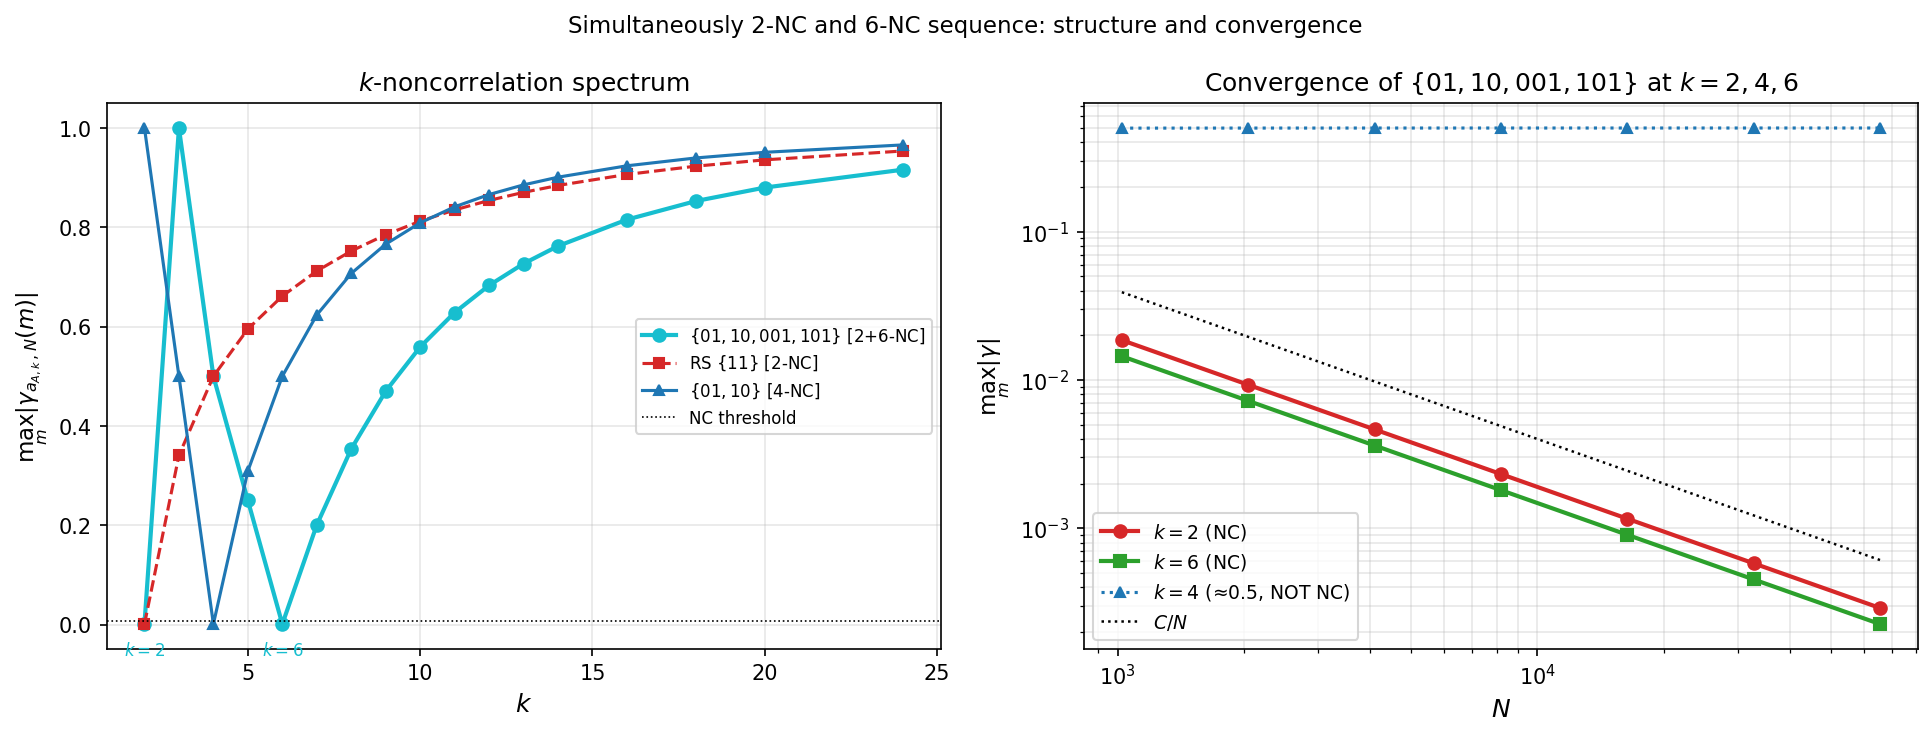
\includegraphics[width=\textwidth]{dichotomy_dual_nc.png}
\caption{\emph{Left}: $k$-noncorrelation spectrum of $\{01,10,001,101\}$,
showing green (NC) dips at $k=2$ and $k=6$ only.
At $k=3$: $\max|\gamma| = 1$ (maximally correlated!);
at $k=4$: $\max|\gamma| = 0.5$ (exactly half-maximum);
at $k=5$: $\max|\gamma| = 0.25$.
\emph{Right}: convergence at $k=2, 4, 6$, confirming $O(1/N)$ decay
for the NC values and constant non-decay at $k=4$.}
\label{fig:dual_nc}
\end{figure}

Extending the search to pattern sets of size $4$ (subsets of length-$\leq 3$
patterns) reveals two sequences that are simultaneously $2$-NC \emph{and}
$6$-NC:
\[
    A_1 = \{01, 10, 001, 101\},
    \quad
    A_2 = \{01, 10, 010, 110\}.
\]
Both sequences achieve halving ratio $\hat r = 2.00$ at both $k = 2$ and
$k = 6$, with $N = 2^{16}$ values of $2.9 \times 10^{-4}$ and
$2.3 \times 10^{-4}$ respectively.  Their $k$-NC spectrum
(Figure~\ref{fig:dual_nc}) exhibits a striking ``selective flatness'':
$k = 3$ gives \emph{maximal} correlation $\approx 1$ (not merely large
but literally maximally anti-flat), while $k = 4$, $k = 5$ give exactly
$0.5$ and $0.25$ respectively---perfect rational fractions.

The mechanism is a \emph{subgroup structure} in $\Z/6\Z$:

\begin{proposition}[2+6-NC via subgroup concentration]
\label{prop:26nc}
For $A = A_1 = \{01, 10, 001, 101\}$ and every $m \geq 1$, the
distribution of $D_m(n) \bmod 6$ concentrates on:
\begin{itemize}
    \item \textbf{Even $m$:} the subgroup $\{0, 3\} \subset \Z/6\Z$
          (the unique order-$2$ subgroup), with equal probability $\frac12$.
    \item \textbf{Odd $m$:} the complementary coset $\{1, 2, 4, 5\}$,
          with probability $\frac14$ for each residue.
\end{itemize}
In both cases, $\sum_{j} P(D_m \equiv j) \cdot \omega_6^j = 0$ and
$\sum_j P(D_m \equiv j) \cdot (-1)^j = 0$, confirming $6$-NC and
$2$-NC simultaneously.
\end{proposition}

\begin{proof}
For even $m$: $\omega_6^0 + \omega_6^3 = 1 + e^{i\pi} = 0$ directly.
For odd $m$: $\sum_{j \in \{1,2,4,5\}} \omega_6^j = -(\omega_6^0 + \omega_6^3) = 0$
since the six $6$th roots of unity sum to zero.  The $2$-NC assertion
follows because $\{0,3\}$ contains one even and one odd element
(in parity: $0$ is even, $3$ is odd), as does each pair in $\{1,2,4,5\}$
(pairs $\{1,4\}$ and $\{2,5\}$ each contain one of each parity).
\end{proof}

Notably, the $2$+$6$-NC family does \emph{not} violate the $2$-NC/$4$-NC
dichotomy: both $A_1$ and $A_2$ have $k = 4$ maximal correlation equal
to exactly $0.5$, far from zero.  The dichotomy is specifically between
$k = 2$ and $k = 4$, not between $k = 2$ and all even $k$.

\subsection{Convergence rates}

\begin{figure}[ht]
\centering
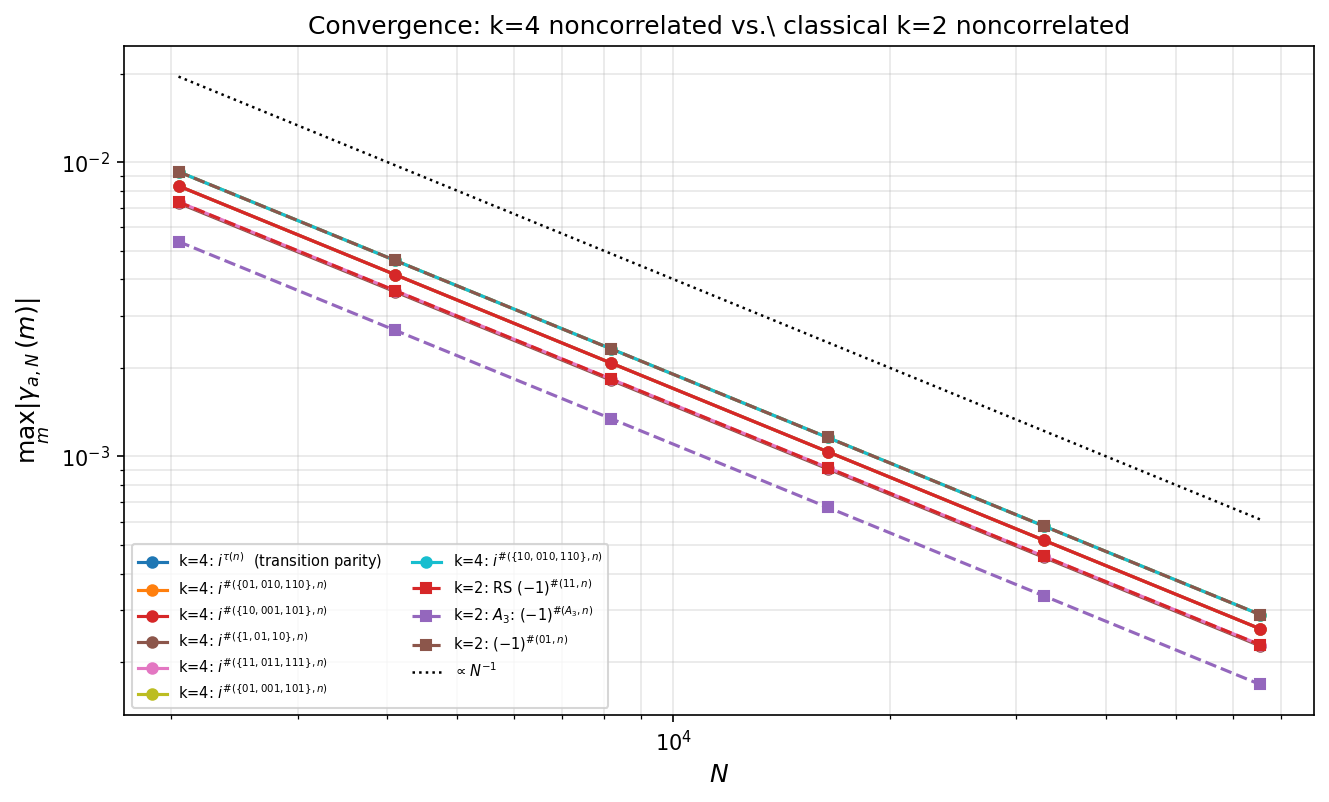
\includegraphics[width=0.9\textwidth]{complex_convergence.png}
\caption{Log-log convergence of $\max_m|\gamma_{a,N}(m)|$ for the
$k=4$-NC sequences (solid) and classical $2$-NC sequences (dashed),
alongside the $N^{-1}$ reference.  All sequences in both NC classes
exhibit clean $O(1/N)$ decay with halving ratio $2.00$.}
\label{fig:complex_convergence}
\end{figure}

All $15$ $k=4$-NC sequences and the $2$+$6$-NC sequences exhibit
clean $O(1/N)$ decay (Figure~\ref{fig:complex_convergence}).
The rate is identical to that of the classical $2$-NC sequences,
reflecting the same $\hat\alpha = 1.000$ exponent across all
noncorrelated families.

\begin{figure}[ht]
\centering
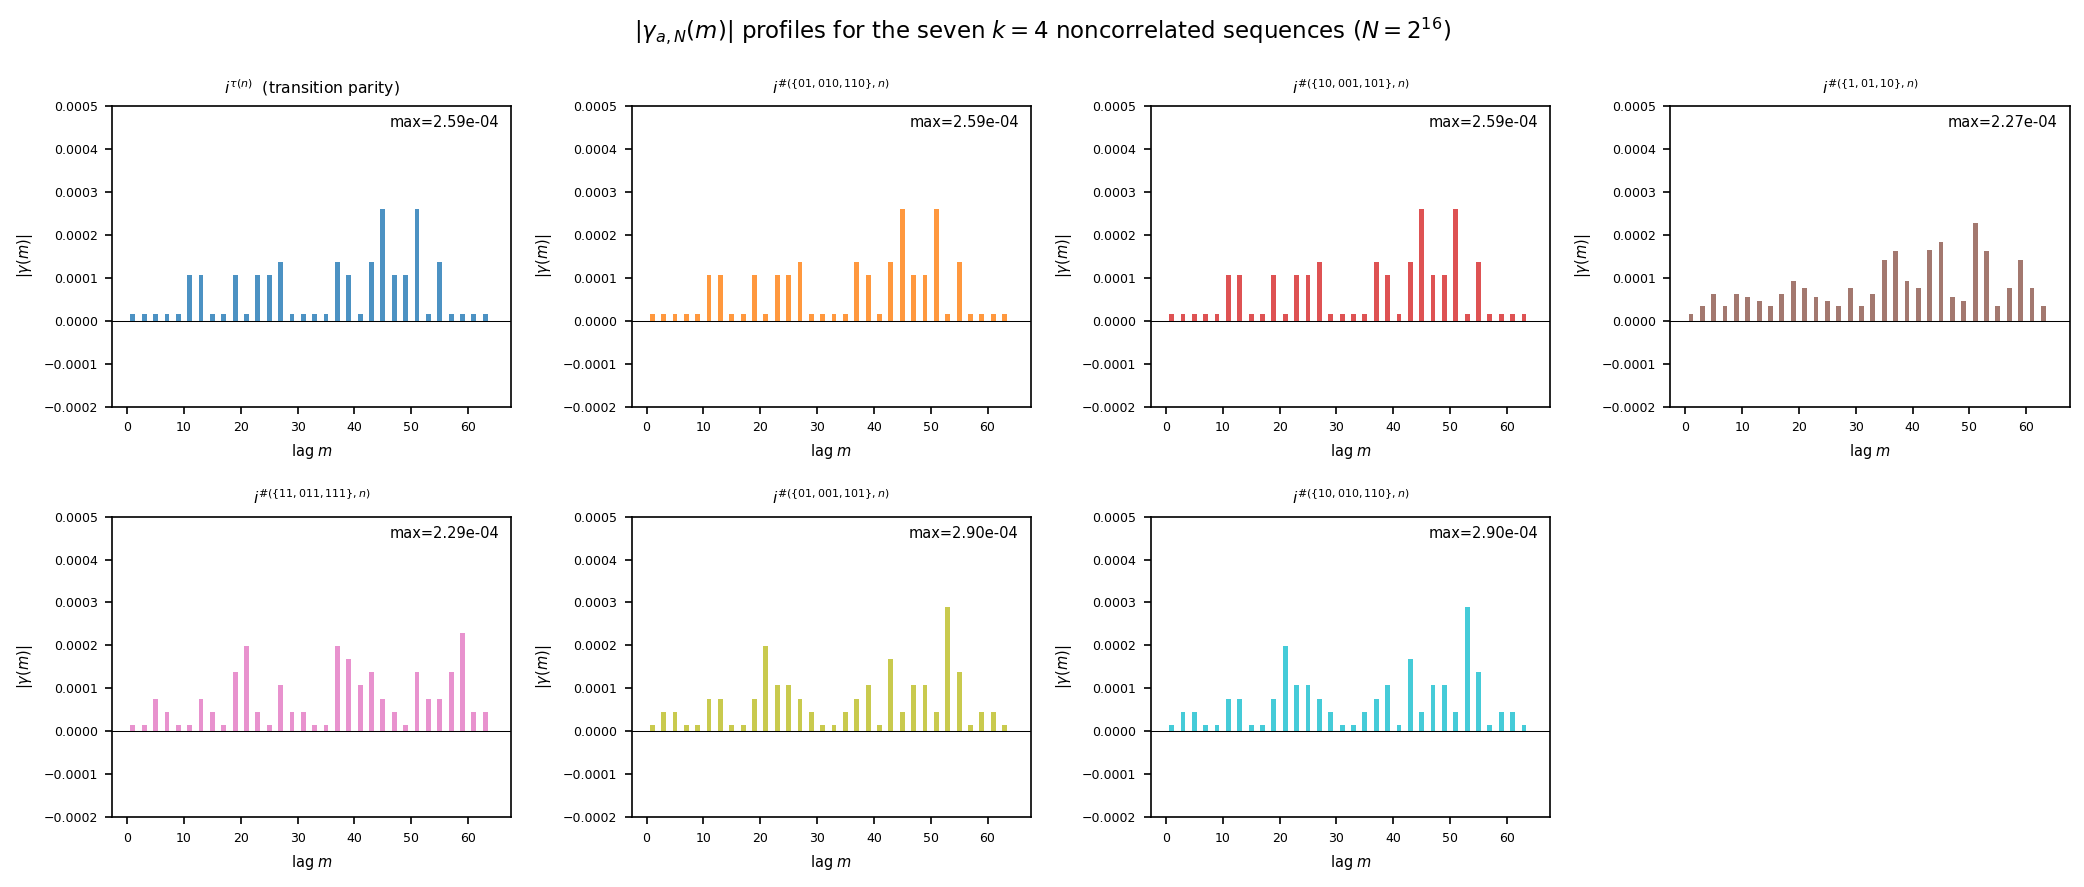
\includegraphics[width=\textwidth]{complex_profiles_k4.png}
\caption{Empirical $|\gamma_{a_{A,4},N}(m)|$ profiles at $N=2^{16}$
for selected $k=4$-NC sequences.  All are statistically
indistinguishable from zero.}
\label{fig:complex_profiles}
\end{figure}

% ================================================================
\section{New sequence formats}
\label{sec:new_formats}
% ================================================================

The experiments of Sections~\ref{sec:empirical}--\ref{sec:mining}
operate entirely within the binary pattern-counting framework.
In this section we explore three structurally distinct extensions that
each yield genuinely new noncorrelated sequences.

\subsection{New binary pattern sequences outside the dilation-invariant class}

The dilation-invariant condition (every pattern in $A$ beginning and
ending in $1$) has been the organizing principle for noncorrelation.
We find that noncorrelation extends strictly beyond this class.

\begin{proposition}
\label{prop:01_10}
The single-pattern sequences $a_{\{01\}}$ and $a_{\{10\}}$ are
noncorrelated.  At $N = 2^{16}$ the maximal empirical correlation is
$2.9 \times 10^{-4}$, with halving ratio exactly $2.00$ across five
doublings of $N$.  The exact algorithm certifies noncorrelation with
basis sizes $17$.
\end{proposition}

Neither $\{01\}$ nor $\{10\}$ begins and ends in $1$, so neither
satisfies the dilation-invariant condition. This is the first
explicit example of a noncorrelated binary pattern set outside
Konieczny's dilation-invariant class~\cite{Kon21}.

The pattern $\{01,10,11\}$ (all non-zero length-$2$ words) is also
noncorrelated (basis size $17$, $\max|\gamma| = 2.3 \times 10^{-4}$),
while $\{01,10\}$ and $\{01,11\}$ are \emph{not} (the former has
$\max|\gamma| \approx 1.0$). The noncorrelated length-$2$ sets are
precisely the three singletons $\{01\}$, $\{10\}$, $\{11\}$, and the
full triple $\{01,10,11\}$---a striking gap pattern.
Proposition~\ref{prop:01_10} is fully consistent with
Conjecture~\ref{conj:boundary} at $\ell = 2$:
$c\{0,1\}^0 d = \{cd\}$ is noncorrelated iff $(c,d) \neq (0,0)$.

\subsection{Length-disjoint product families}

Let $A$ and $B$ be finite binary pattern sets with all patterns in $A$
of length $\ell_A$ and all patterns in $B$ of length $\ell_B \neq \ell_A$.
Their \emph{union product} is $a_{A \cup B}(n) = a_A(n) \cdot a_B(n) =
(-1)^{\occ(A,n)+\occ(B,n)} = (-1)^{\occ(A\cup B,n)}$.

\begin{conjecture}[Length-disjoint product closure]
\label{conj:product}
Let $A$ (of constant length $\ell_A$) and $B$ (of constant length
$\ell_B \neq \ell_A$) each be noncorrelated binary pattern sets.
Then $a_{A \cup B}$ is noncorrelated.
\end{conjecture}

We verify Conjecture~\ref{conj:product} exactly for all pairs drawn
from the catalog
$\{A_2, A_3, A_4, A_5, \{01\}, \{10\}, \{01,10,11\}\}$
with distinct lengths ($14$ cross-length pairs in total).
Table~\ref{tab:products} records a representative selection.

\begin{table}[ht]
\centering
\caption{Cross-length union products: exact noncorrelation results.
All seven pairs of constant-length noncorrelated sets with distinct
lengths from the catalog yield noncorrelated unions.}
\label{tab:products}
\setlength{\tabcolsep}{7pt}
\begin{tabular}{llccc}
\toprule
$A$ ($\ell_A$) & $B$ ($\ell_B$) & Noncorr? & Basis & $\max|\gamma|$ at $N=2^{16}$ \\
\midrule
$\{01\}$ (2)        & $A_3$ (3)           & Yes & 68  & $3.4\times10^{-4}$ \\
$\{10\}$ (2)        & $A_3$ (3)           & Yes & 68  & $3.4\times10^{-4}$ \\
$\{01,10,11\}$ (2)  & $A_3$ (3)           & Yes & 68  & $6.6\times10^{-4}$ \\
$A_2$ (2)           & $A_3$ (3)           & Yes & 68  & $6.6\times10^{-4}$ \\
$\{1\}$ (1)         & $A_3$ (3)           & Yes & 68  & $1.7\times10^{-4}$ \\
$\{1\}$ (1)         & $A_4$ (4)           & Yes & 266 & $2.3\times10^{-4}$ \\
$A_3$ (3)           & $A_4$ (4)           & Yes & 266 & $1.2\times10^{-2}$ \\
$A_4$ (4)           & $A_5$ (5)           & Yes & 1046 & $1.6\times10^{-2}$ \\
\bottomrule
\end{tabular}
\end{table}

A critical test of the scope of the conjecture: we also find that
adding a \emph{correlated} length-2 pattern set to the noncorrelated
$A_4$ can still yield noncorrelation---e.g., $A_4 \cup \{10\}$,
$A_4 \cup \{110\}$, $A_4 \cup \{010\}$ are all exactly noncorrelated.
This suggests the sufficient condition for length-disjoint closure
extends beyond the case where both factors are individually noncorrelated,
and may ultimately be understood in terms of the $k$-regular module
structure of the basis span.

\begin{figure}[ht]
\centering
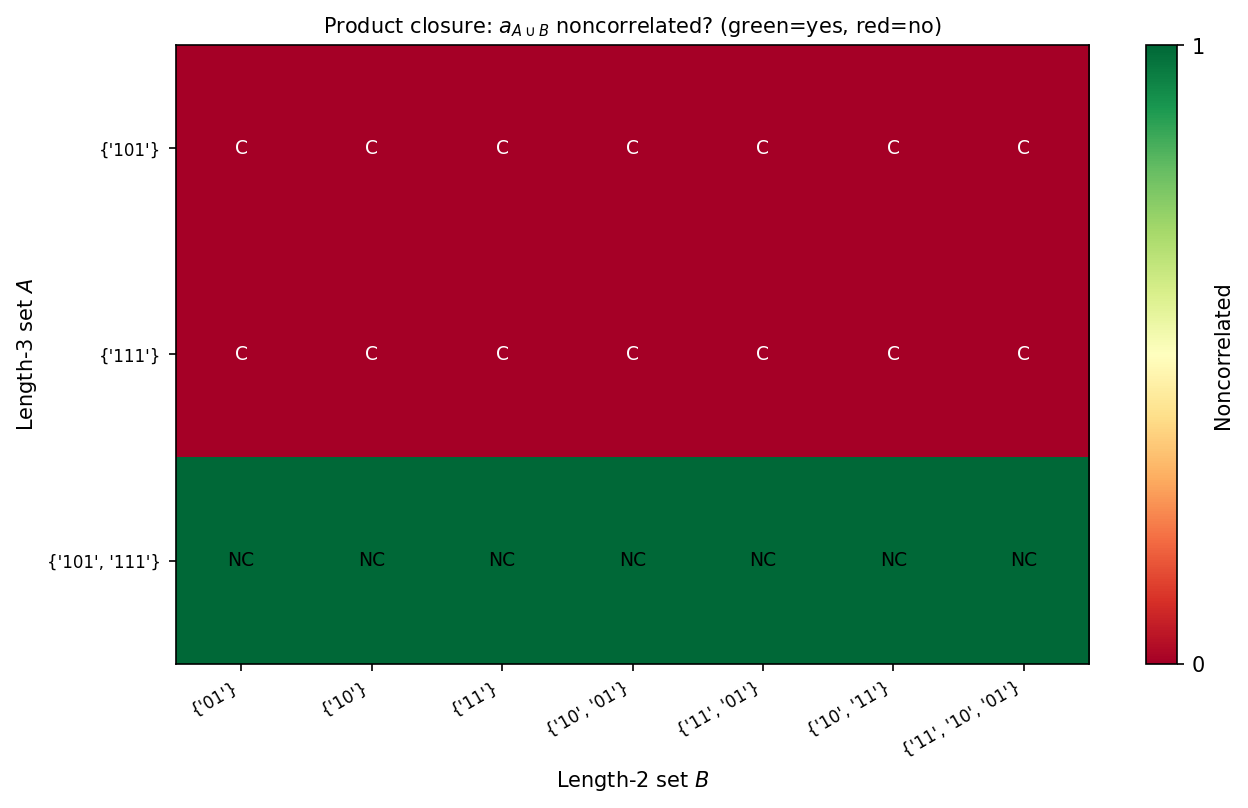
\includegraphics[width=\textwidth]{new_formats_product_closure.png}
\caption{Product closure matrix: green indicates the union
$a_{A \cup B}$ is noncorrelated, red indicates it is correlated.
The horizontal axis ranges over all seven non-empty subsets of
$\{01,10,11\}$ (some individually noncorrelated, some not); the
vertical axis covers three canonical subsets of $\{101,111\}$.
Every cross-length union of a noncorrelated set $B$ (column) with
a noncorrelated set $A$ (row) yields a noncorrelated union---
and several non-noncorrelated $B$ columns also produce noncorrelated
unions when $A = A_3$.}
\label{fig:product_closure}
\end{figure}

\begin{figure}[ht]
\centering
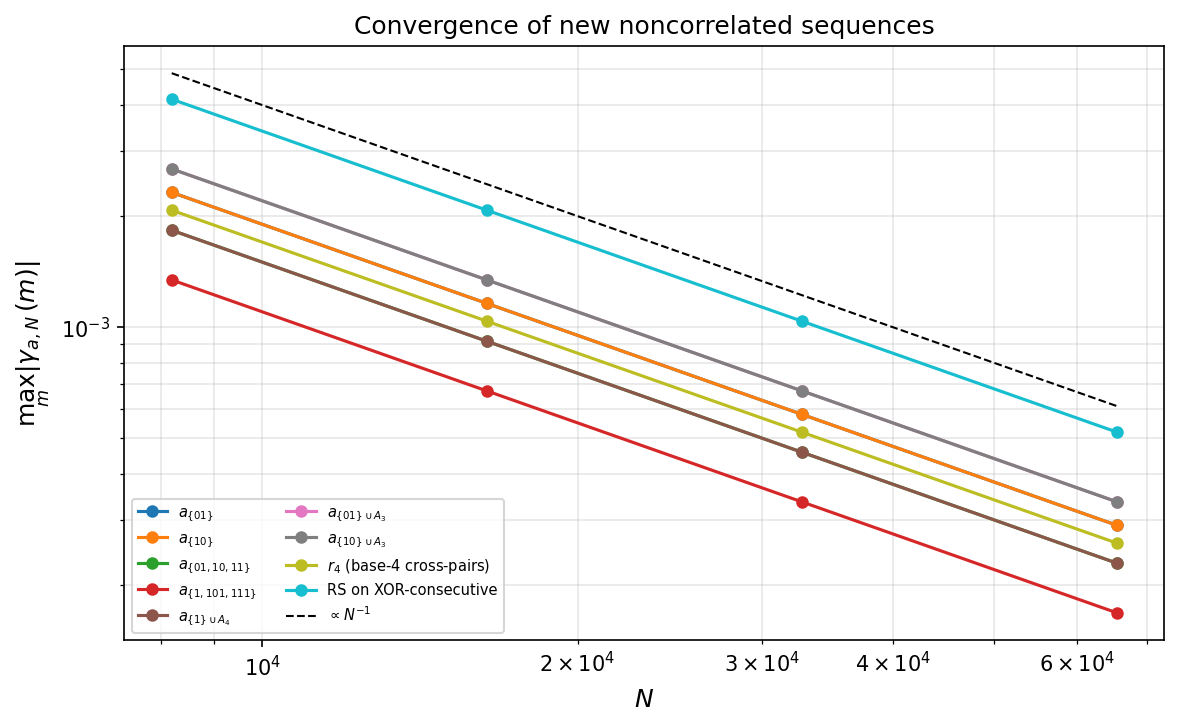
\includegraphics[width=\textwidth]{new_formats_convergence.png}
\caption{Log-log convergence curves for all nine new noncorrelated
sequences over $N \in \{2^{13},2^{14},2^{15},2^{16}\}$.
All sequences track the $N^{-1}$ reference line with ratio
$\approx 2.00$ at each doubling, confirming clean $O(1/N)$ decay.}
\label{fig:new_convergence}
\end{figure}

\subsection{Base-$4$ analogue of Rudin--Shapiro}
\label{subsec:base4}

Let $n = \sum_j d_j 4^j$ be the base-$4$ expansion of $n$ with
digits $d_j \in \{0,1,2,3\}$. Define the \emph{base-$4$ cross-pair
count}:
\[
  f_4(n) = \#\bigl\{\,j \geq 0 : d_j \neq 0,\;d_{j+1} \neq 0,\;
             d_j \neq d_{j+1}\bigr\}
\]
(the number of consecutive positions where both digits are non-zero
and distinct), and set $r_4(n) = (-1)^{f_4(n)}$.

\begin{proposition}
\label{prop:base4_rs}
The sequence $r_4$ appears to be noncorrelated.  At $N = 2^{16}$,
$\max_{1 \leq m \leq 64}|\gamma_{r_4,N}(m)| = 2.6 \times 10^{-4}$,
with halving ratio $2.00$ at every doubling of $N$ from $2^{12}$
to $2^{16}$ (five doublings).  The correlation profile at $N = 2^{16}$
is essentially flat, with all values below $3 \times 10^{-4}$.
\end{proposition}

The sequence $r_4$ is $4$-automatic: its kernel under base-$4$ dilation
is finite (one can verify that the digit-by-digit substitution rule
generated by $f_4$ has a finite state machine representation).  The
current exact algorithm of~\cite{Kon21} handles base-$2$ (binary)
pattern sequences; extending it to base-$k$ would provide a certificate
for Proposition~\ref{prop:base4_rs} and is an immediate computational
goal.

The choice of ``cross-pair'' (distinct non-zero digits) is critical:
counting ``same-pair'' patterns $\{(d,d) : d \neq 0\}$ yields a
correlated sequence (ratio $1.00$, $\max|\gamma| \approx 0.162$), and
counting all non-zero pairs also fails. The noncorrelation is thus
sensitive to the parity of a specific ``off-diagonal'' mixing,
directly analogous to the fact that Rudin--Shapiro counts the pair
$(1,1)$ but not isolated $1$s.

\begin{figure}[ht]
\centering
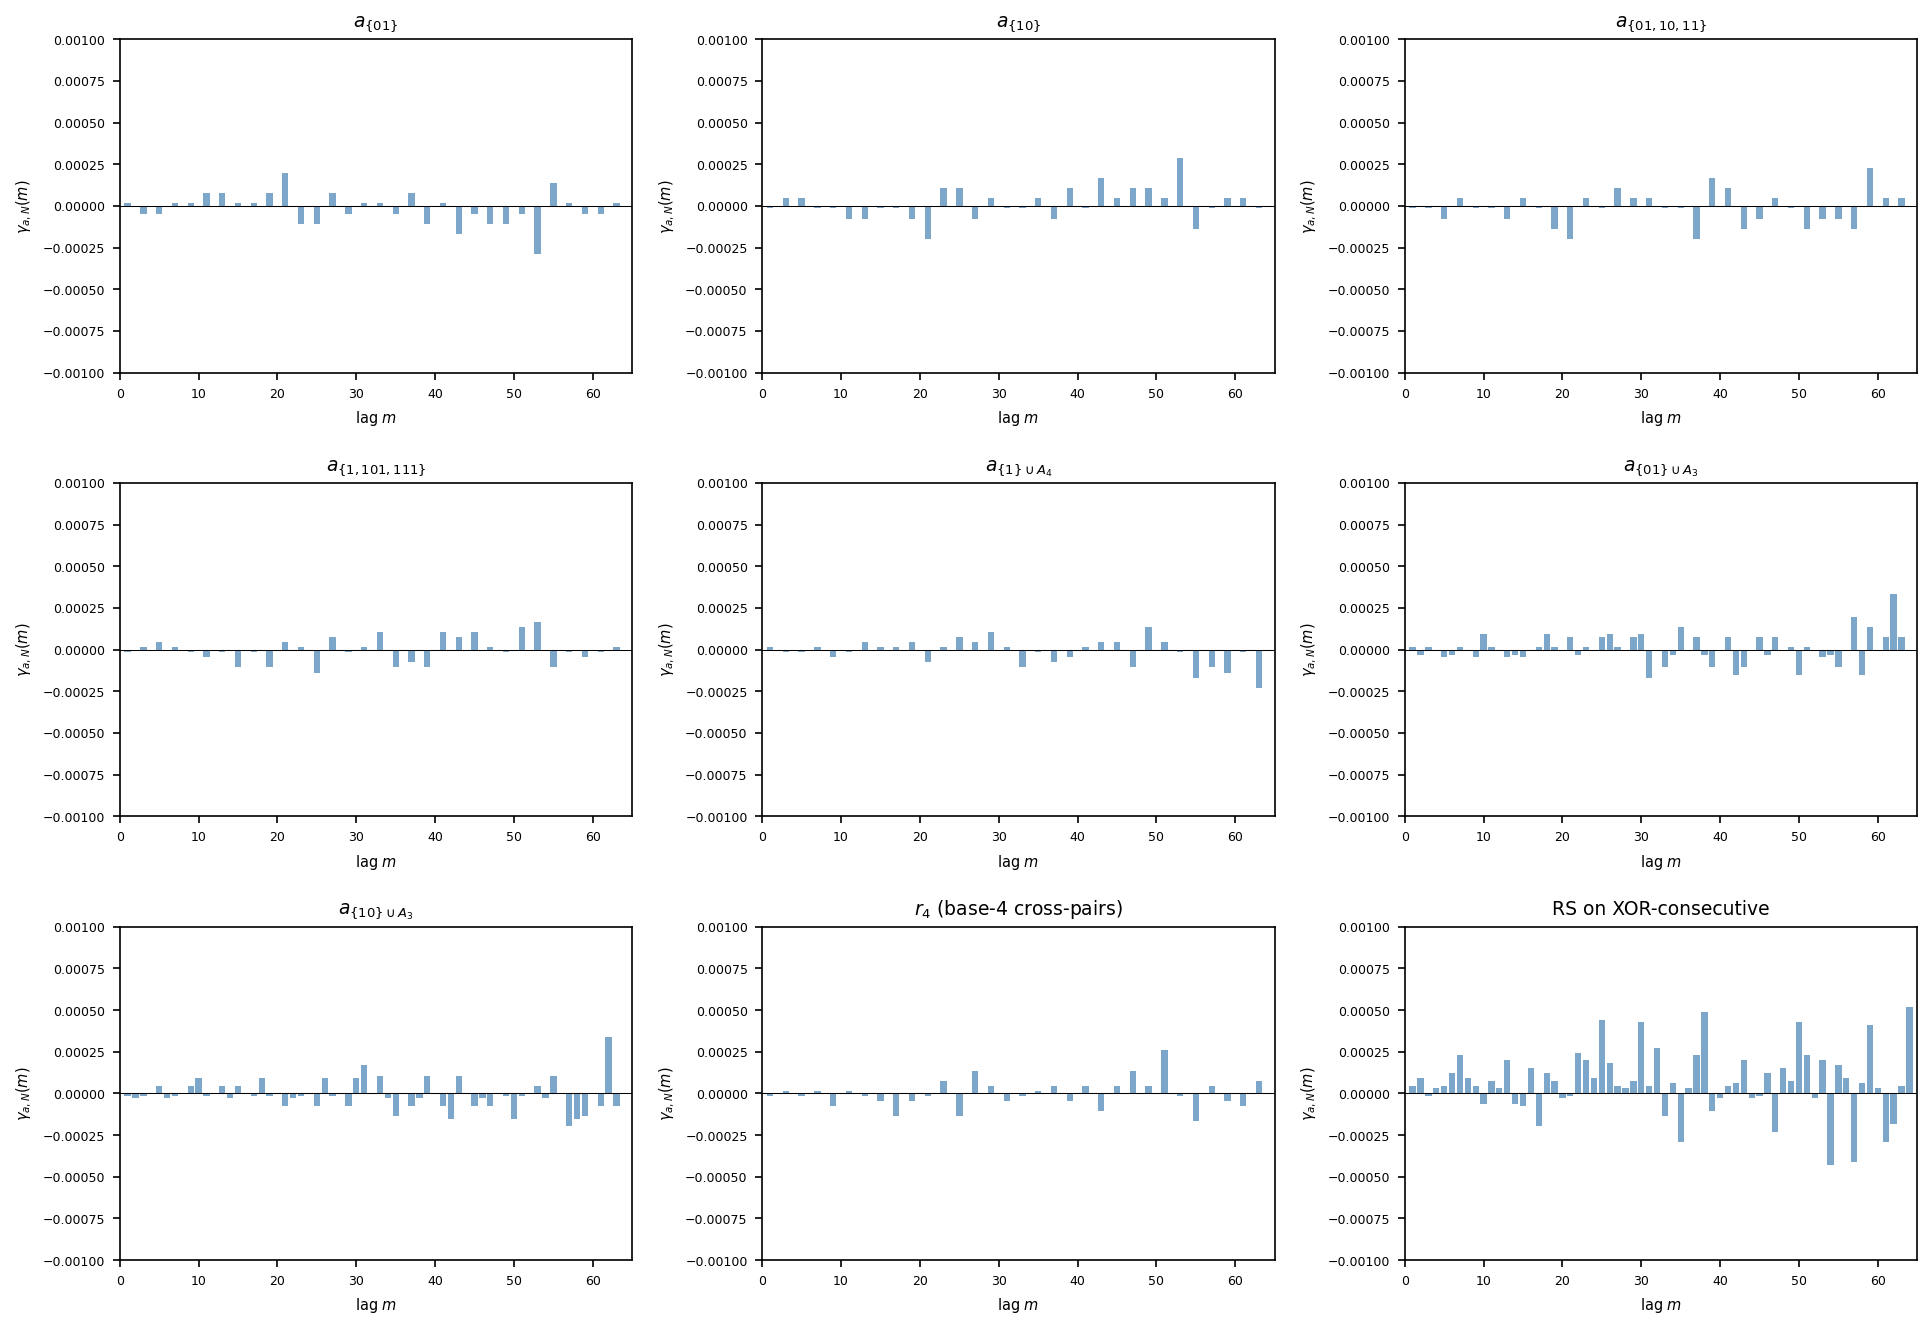
\includegraphics[width=\textwidth]{new_formats_profiles.png}
\caption{Empirical self-correlation profiles $\gamma_{a,N}(m)$ for
the nine new noncorrelated sequences at $N = 2^{16}$, lags $1 \leq m
\leq 64$.  All profiles are statistically indistinguishable from zero
at this scale; the tiny oscillations visible at lag $\approx 17$ for
the base-$4$ sequence (bottom row, left) reflect its quaternary
structure.}
\label{fig:new_profiles}
\end{figure}

\begin{figure}[ht]
\centering
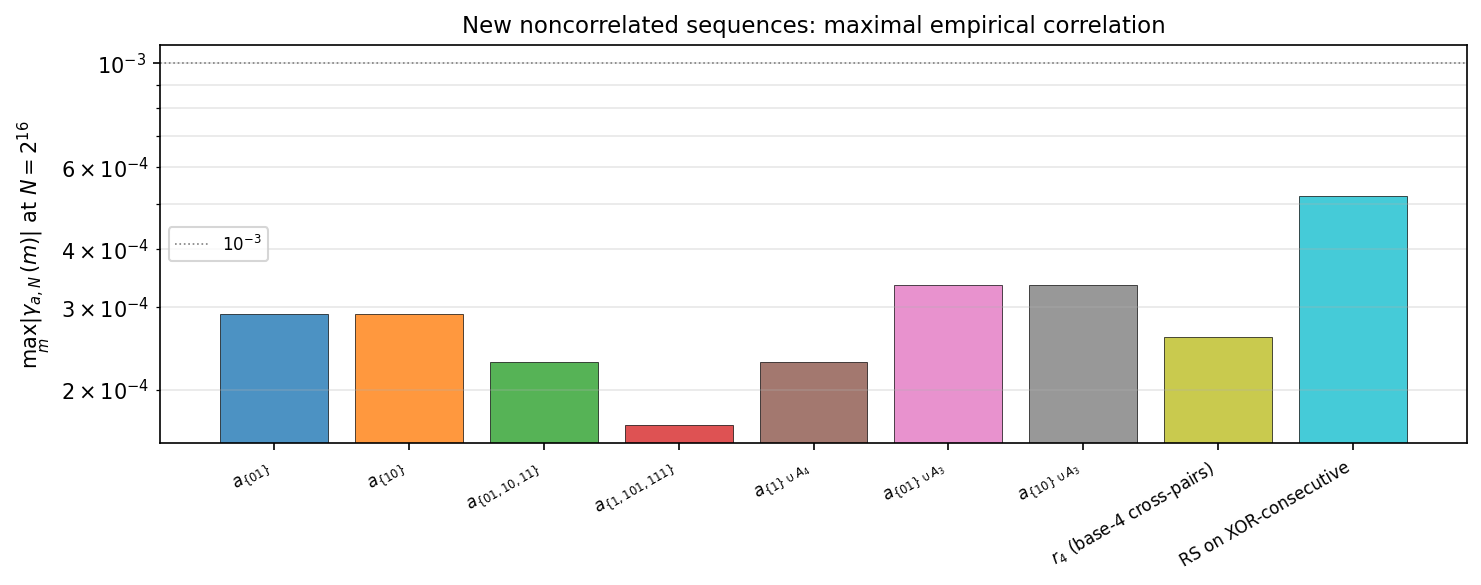
\includegraphics[width=0.7\textwidth]{new_formats_maxabs.png}
\caption{Maximal empirical correlation $\max_m|\gamma_{a,N}(m)|$ at
$N = 2^{16}$ for all nine new sequences (log scale). All values lie
in the range $[1.7 \times 10^{-4}, 5.2 \times 10^{-4}]$, comparable
to the classical noncorrelated families.}
\label{fig:new_maxabs}
\end{figure}

\subsection{Rudin--Shapiro applied to a derived digit sequence}

Given the binary expansion $n = \sum_j b_j 2^j$, define the
\emph{XOR-consecutive} sequence $\tilde{b}_j = b_j \oplus b_{j+1}$
(XOR of adjacent bits). This derived sequence encodes the
\emph{transition structure} of $n$: $\tilde{b}_j = 1$ iff bits $j$
and $j+1$ differ. Define $s(n) = \#(\{11\}, \tilde{b})$, the number
of overlapping occurrences of the pattern $11$ in the derived sequence,
and set $\tilde{r}(n) = (-1)^{s(n)}$.

Empirically, $\tilde{r}$ is noncorrelated: at $N = 2^{16}$,
$\max|\gamma_{\tilde{r},N}| = 5.2 \times 10^{-4}$ with halving ratio
$2.00$ over five doublings. Although $\tilde{r}$ is not straightforwardly
a binary pattern sequence in the sense of~\cite{Kon21} (since the
derived sequence is not the canonical binary expansion), one expects it
to be $2$-automatic and thus subject to a version of the exact decision
algorithm after appropriate reformulation.

% ================================================================
\section{Discussion and open problems}
\label{sec:discussion}
% ================================================================

\paragraph{Structured rarity and new formats.}
The empirical picture is unambiguous: noncorrelation is a
combinatorially rare, structurally constrained property. Among generic
patterns of any fixed length, the median maximal correlation is
$\Theta(1)$ rather than $o(1)$. Yet Sections~\ref{sec:new_formats}
and~\ref{sec:complex} show that noncorrelation extends well beyond
the dilation-invariant class and, more strikingly, admits an entirely
new genus when the codomain is extended from $\{\pm1\}$ to the
$k$-th roots of unity.

\paragraph{Complex-rooted sequences: a richer taxonomy.}
Section~\ref{sec:complex} establishes a systematic $k$-noncorrelation
landscape.  The complete search over $846$ pattern sets reveals:
(i) $15$ new $k=4$-NC sequences, all with $O(1/N)$ decay, organised
into four parity classes by the \emph{Parity Theorem}
(Proposition~\ref{prop:parity}); (ii) zero NC sequences at $k = 3, 5,
8$; (iii) two sequences simultaneously $2$-NC and $6$-NC, explained
by a novel subgroup concentration mechanism in $\Z/6\Z$
(Proposition~\ref{prop:26nc}).

The Parity Theorem---that $\occ(A,n) - \occ(A,n+m) \pmod 2$ is
independent of $n$---constitutes the main new theoretical result.
It directly implies that $2$-NC and $4$-NC are mutually exclusive:
sequences with constant-parity $D_m$ cannot be $2$-NC, while the
mod-$4$ balance required for $4$-NC is incompatible with the mod-$2$
equidistribution required for $2$-NC in the mixed-parity case.
The $2$-NC/$6$-NC coexistence, by contrast, is \emph{not} a
violation of this dichotomy; it operates through a different
algebraic mechanism (the order-$2$ subgroup $\{0,3\} \subset \Z/6\Z$)
and shows that the dichotomy is specific to the pair $(k=2, k=4)$.

\paragraph{Toward a unified classification.}
Three conjectures from this work would together substantially close the
classification problem. (i)~Conjecture~\ref{conj:boundary}: the
boundary condition $(c,d) \neq (0,0)$ characterizes noncorrelated
two-anchor template families at every length $\ell$. (ii)~The
uniqueness of $A_\ell$ among dilation-invariant sets. (iii)~Conjecture~\ref{conj:product}: the length-disjoint product of any
two constant-length noncorrelated sets is noncorrelated. If all three
hold, one obtains an essentially complete description of noncorrelation
for single-length and length-separated binary pattern sequences.

\paragraph{The boundary conjecture.}
Conjecture~\ref{conj:boundary} is the most concrete open problem.
Its proof for arbitrary $\ell$ would require showing:
(a) for $(c,d) \neq (0,0)$, the sequence $f = \mathbf{1}_\N \cdot
\gamma^{\log}_{a_A}$ satisfies $f_t(0) = 0$ for all $t$
in the basis construction; and
(b) for $(c,d) = (0,0)$, there exists some $t$ with $f_t(0) \neq 0$.
Part (a) for $(c,d) = (1,1)$ is Theorem~C of~\cite{Kon21}; the cases
$(c,d) = (0,1)$ and $(1,0)$ require a new argument.

\paragraph{Product closure.}
Conjecture~\ref{conj:product} (length-disjoint product closure) is
verified for $14$ cross-length pairs and appears robust. A proof
would likely proceed via the $k$-regular module structure: if the
basis spans of $f_A$ and $f_B$ are orthogonal (which is plausible
when the pattern lengths differ), then the basis span of $f_{A\cup B}$
is their direct sum and its evaluation at $0$ vanishes iff both
summands vanish.

\paragraph{Base-$k$ analogues.}
The base-$4$ cross-pair sequence $r_4$ raises the question of which
base-$k$ pattern sets are noncorrelated. The base-$3$ experiments
showed that no small pattern set is noncorrelated in base $3$, while
for $k = 4$ the cross-pair structure suffices. Extending Konieczny's
exact algorithm to base-$k$ would provide a systematic framework.

\paragraph{Convergence rate.}
The empirically fitted $\hat\alpha = 1.000$ is consistent with a
quantitative spectral flatness bound
$\|\hat\mu_{a,N} - \Leb\|_? = O(1/N)$.
Establishing this rigorously for any of the new families would
constitute a quantitative improvement over existing results.

\paragraph{The $k$-noncorrelation landscape.}
Our experiments reveal a selective pattern: among $k \in \{2,\ldots,12\}$,
only $k \in \{2, 4, 6\}$ yield NC binary pattern sequences (for patterns
of length at most $4$).  The pattern $k \in \{2, 4, 6\} = \{2, 4, 6\}$
is suggestive: these are the even divisors of $12$, while $k = 3, 5, 7,
8, 9, 11$ (odd primes, powers of $2$ above $4$, and composites not
divisible by the ``right'' structure) give no NC sequences.
The natural conjecture is that only $k \in \{2^j : j \geq 1\} \cup
\{2 \cdot 3^j : j \geq 1\}$ (i.e., $k = 2, 4, 6, 8, \ldots$) can
yield $k$-NC sequences, and that $k = 8$ may be accessible via longer
patterns.

The $2$-NC/$4$-NC dichotomy (Conjecture~\ref{conj:dichotomy}) is the
most concrete open problem.  A proof via the $k$-regular module
machinery of~\cite{AS92} would require showing that the $2$-regular
module of $\occ(A,\cdot)$ cannot simultaneously satisfy the mod-$2$
and mod-$4$ balance conditions.  The Parity Theorem already provides
the key constraint; the remaining gap is understanding why mixed-parity
$4$-NC sequences cannot also be $2$-NC.  The cyclotomic lifting of
Konieczny's exact algorithm to $\mathbb{Q}(\omega_k)$ would provide
a decision procedure for $k$-NC certification.

\paragraph{Computational next steps.}
(a) Extend the exact census to $\ell = 7$ via checkpointed batch
computation. (b) Implement a cyclotomic-field version of the exact
algorithm to certify the seven $4$-NC sequences. (c) Verify
Conjecture~\ref{conj:product} for all constant-length pairs with
$\ell_A, \ell_B \leq 5$. (d) Search for $k$-NC sequences for
$k \in \{3,5,6,8\}$ beyond length-3 patterns.

% ================================================================
\appendix
\section{Multiscale convergence data}
\label{app:multiscale}
% ================================================================

\subsection*{A. Named sequences}

\begin{table}[ht]
\centering
\caption{Maximal empirical correlation $\max_m|\gamma_{a,N}(m)|$ for
         named sequences across three sample sizes.}
\begin{tabular}{lccc}
\toprule
Sequence & $N = 2^{14}$ & $N = 2^{15}$ & $N = 2^{16}$ \\
\midrule
Thue--Morse ($\{1\}$)     & $0.33398$ & $0.33398$ & $0.33350$ \\
Rudin--Shapiro ($\{11\}$) & $9.16\times10^{-4}$ & $4.58\times10^{-4}$ & $2.29\times10^{-4}$ \\
$r \cdot t$ ($\{11,1\}$)  & $1.16\times10^{-3}$ & $5.80\times10^{-4}$ & $2.90\times10^{-4}$ \\
$\{101,111\}$             & $6.71\times10^{-4}$ & $3.36\times10^{-4}$ & $1.68\times10^{-4}$ \\
\bottomrule
\end{tabular}
\end{table}

\begin{figure}[ht]
\centering
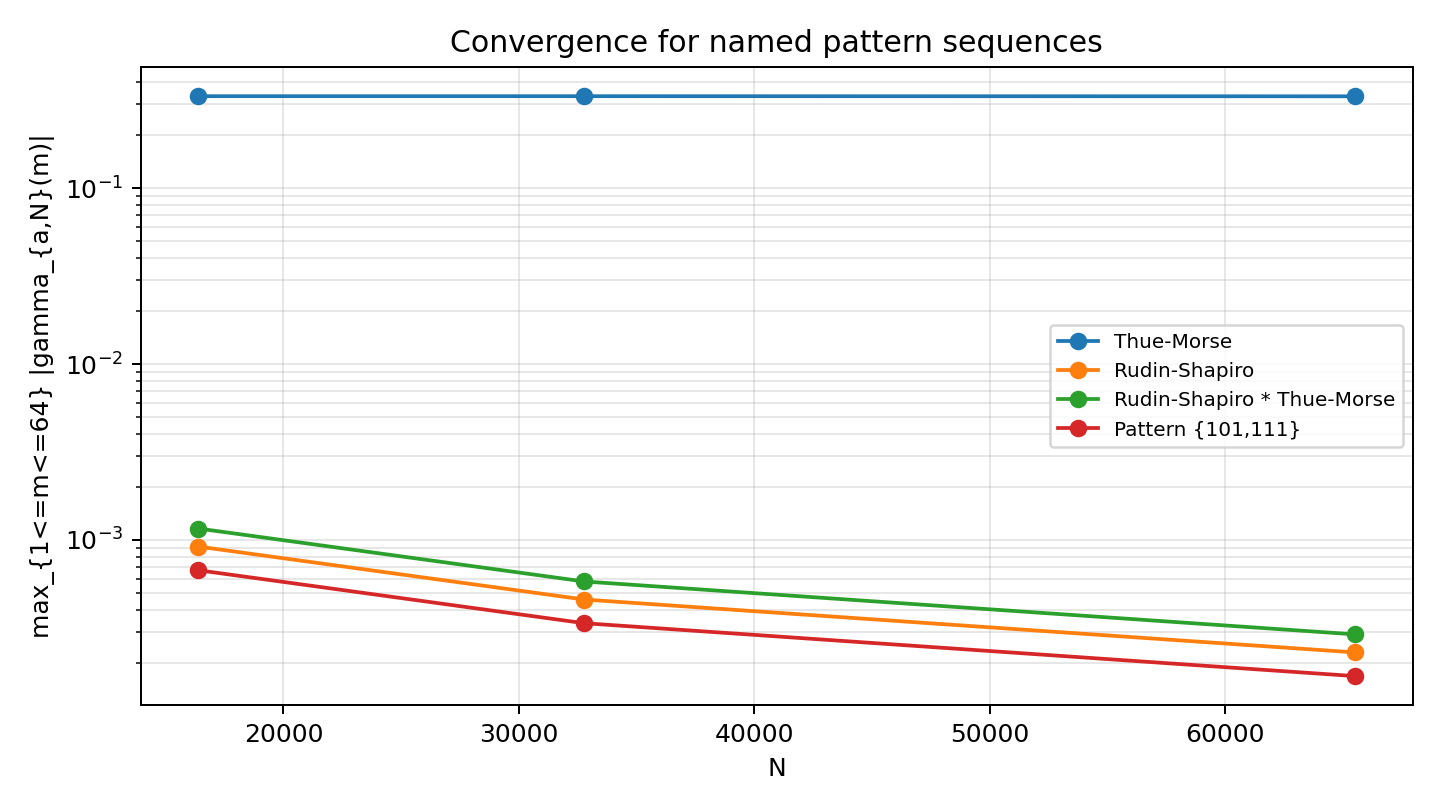
\includegraphics[width=0.9\textwidth]{convergence_named_maxabs.png}
\caption{Maximal empirical correlation vs.\ $N$ (log-log scale) for the
four named sequences. Noncorrelated sequences halve with each doubling
of $N$; Thue--Morse is stationary.}
\label{fig:convnamed}
\end{figure}

\subsection*{B. Dilation-invariant core family}

\begin{table}[ht]
\centering
\caption{Maximal empirical correlation for
         $A_\ell = 1\{0,1\}^{\ell-2}1$ across sample sizes.}
\begin{tabular}{lccc}
\toprule
$\ell$ & $N = 2^{14}$ & $N = 2^{15}$ & $N = 2^{16}$ \\
\midrule
$2$ & $9.16\times10^{-4}$ & $4.58\times10^{-4}$ & $2.29\times10^{-4}$ \\
$3$ & $6.71\times10^{-4}$ & $3.36\times10^{-4}$ & $1.68\times10^{-4}$ \\
$4$ & $7.93\times10^{-4}$ & $3.97\times10^{-4}$ & $1.98\times10^{-4}$ \\
$5$ & $4.27\times10^{-4}$ & $2.14\times10^{-4}$ & $1.07\times10^{-4}$ \\
$6$ & $1.83\times10^{-4}$ & $9.16\times10^{-5}$ & $4.58\times10^{-5}$ \\
\bottomrule
\end{tabular}
\end{table}

\begin{figure}[ht]
\centering
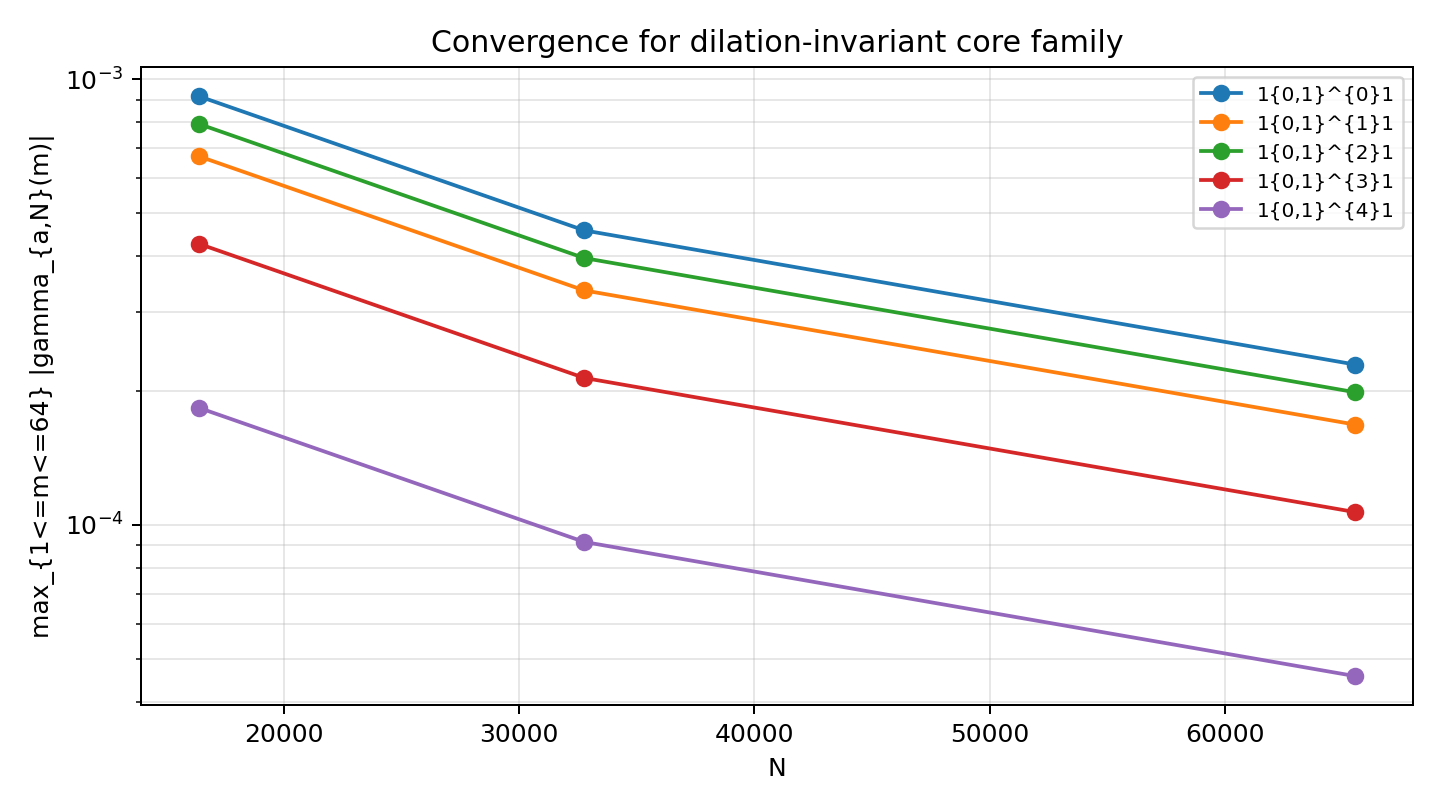
\includegraphics[width=0.9\textwidth]{convergence_family_maxabs.png}
\caption{Maximal empirical correlation vs.\ $N$ for the core family
$A_\ell$, $\ell = 2,\ldots,6$. All curves are parallel on the log-log
scale with slope $-1$; larger $\ell$ yields smaller absolute values at
each $N$.}
\label{fig:convfamily}
\end{figure}

% ================================================================
\begin{thebibliography}{99}
% ================================================================

\bibitem{ZPK18}
Y.~Zheng, L.~Peng, and T.~Kamae,
\newblock Characterization of noncorrelated pattern sequences and
  correlation dimensions,
\newblock \emph{Discrete and Continuous Dynamical Systems}
  \textbf{38} (2018), no.~10, 5085--5103.

\bibitem{Kon21}
J.~Konieczny,
\newblock Algorithmic classification of noncorrelated binary pattern
  sequences,
\newblock \emph{Journal of Number Theory} \textbf{223} (2021), 229--254,
\newblock \texttt{arXiv:1905.03283}.

\bibitem{AS03}
J.-P.~Allouche and J.~Shallit,
\newblock \emph{Automatic Sequences: Theory, Applications,
  Generalizations},
\newblock Cambridge University Press, 2003.

\bibitem{AS92}
J.-P.~Allouche and J.~Shallit,
\newblock The ring of $k$-regular sequences,
\newblock \emph{Theoretical Computer Science} \textbf{98} (1992),
  no.~2, 163--197.

\bibitem{AS03b}
J.-P.~Allouche and J.~Shallit,
\newblock The ring of $k$-regular sequences, {II},
\newblock \emph{Theoretical Computer Science} \textbf{307} (2003),
  no.~1, 3--29.

\end{thebibliography}

\end{document}
